\documentclass[fleqn]{article}
\usepackage[utf8]{inputenc}
\usepackage{graphicx}
\usepackage{geometry}
\usepackage[fleqn]{amsmath}
\usepackage{tikz}
\usepackage{grffile}
\usepackage{hyperref}
\usepackage{epstopdf}
\usepackage{longtable}
\usepackage{subcaption}
\graphicspath{{}}
\newgeometry{left=3cm, top=2cm, bottom=2cm}
\newcommand{\myparagraph}[1]{\paragraph{#1}\mbox{}\\}
\title{EE6130 Machine Learning for Computer Vision\\ Assignment-3 \\(Depth Estimation from a Stereo Pair))}
\author{Arulkumar S (CS15S023) }
\date{$12^{th}$ May 2016}

\begin{document}
\tracingall
\maketitle


\section{Using simple cost function}
\subsection{map (black \& white image)}
The disparity images found for various patch sizes are given below:
\begin{figure}[!ht]
\begin{subfigure}{0.3\textwidth}
\centering
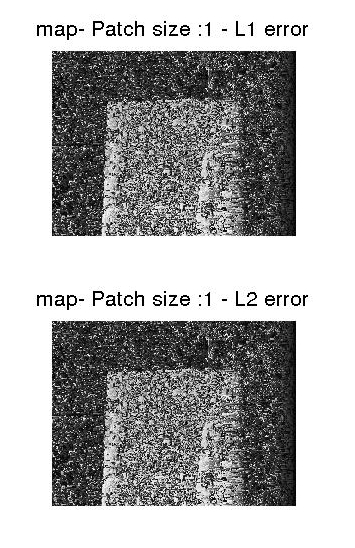
\includegraphics[scale=0.3]{./pics/map_disparity_patchsize_1.jpg}
\caption{Patch size 1}
\end{subfigure}%
 \begin{subfigure}{0.3\textwidth}
 \centering
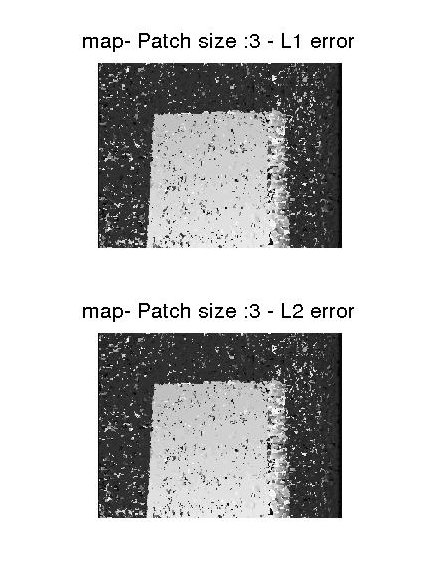
\includegraphics[scale=0.3]{./pics/map_disparity_patchsize_3.jpg}
\caption{Patch size 3}
\end{subfigure}%
 \begin{subfigure}{0.3\textwidth}
 \centering
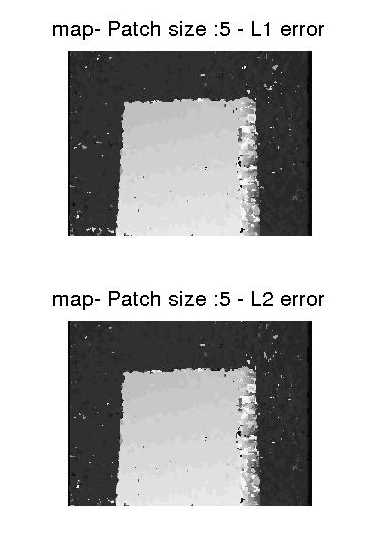
\includegraphics[scale=0.3]{./pics/map_disparity_patchsize_5.jpg}
\caption{Patch size 5}
\end{subfigure}
\begin{subfigure}{0.3\textwidth}
 \centering
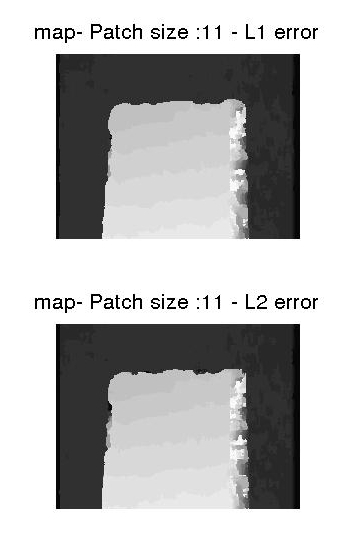
\includegraphics[scale=0.3]{./pics/map_disparity_patchsize_11.jpg}
\caption{Patch size 11}
\end{subfigure}%
\begin{subfigure}{0.3\textwidth}
\centering
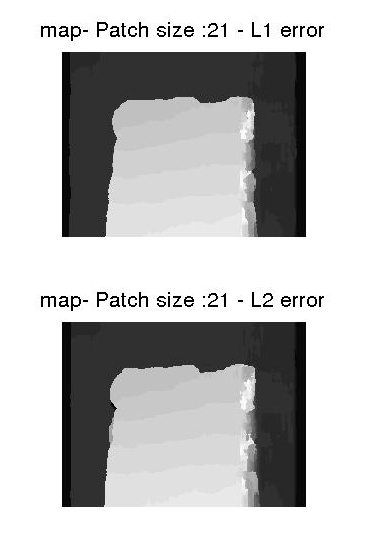
\includegraphics[scale=0.3]{./pics/map_disparity_patchsize_21.jpg}
\caption{Patch size 21}
\end{subfigure}%
\end{figure}

\clearpage
\subsubsection{L1 error vs. L2 error}
\begin{figure}[!ht]
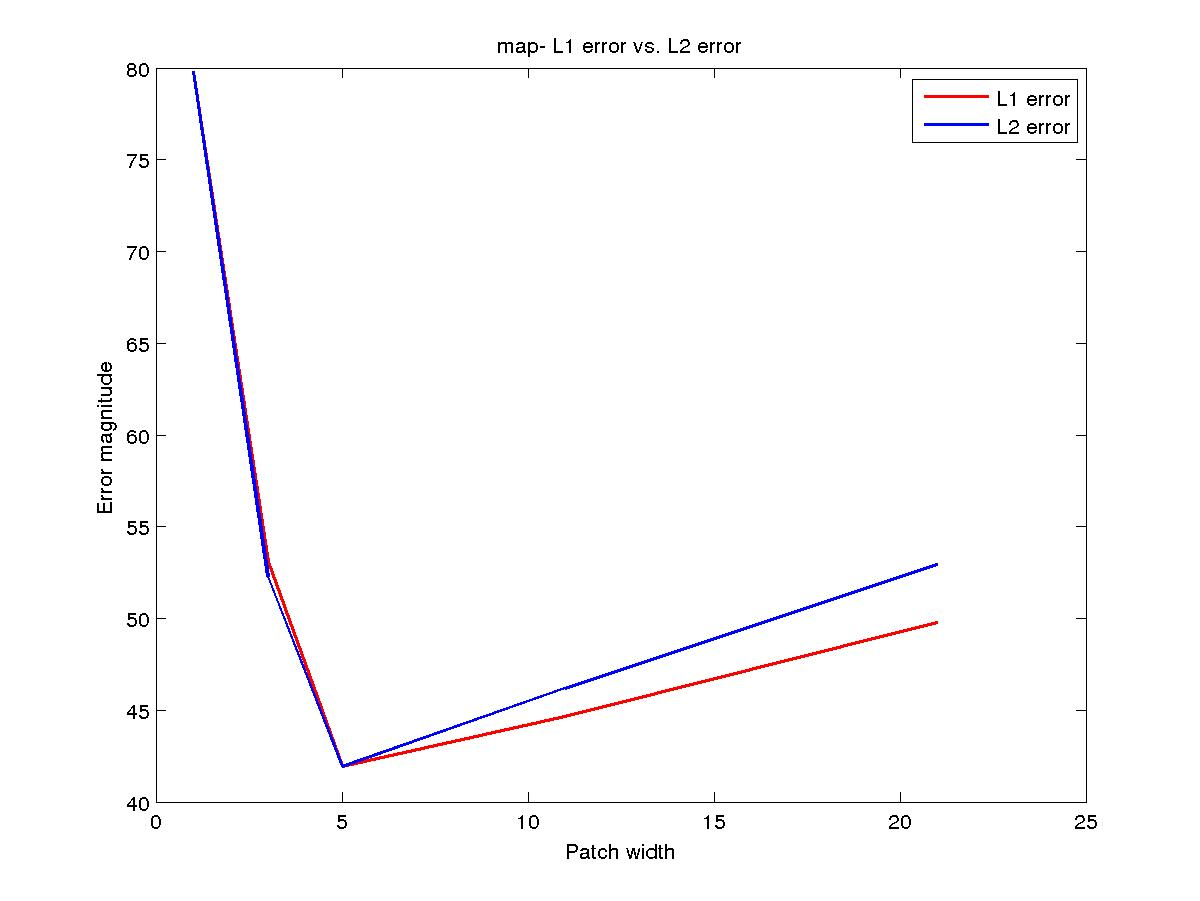
\includegraphics[scale=0.3]{./pics/map_error_vs_patchsize.jpg}
\caption{The L1 error and L2 error starts reducing when the patch size is increased and gives minimum error at patch size of 5. 
then, the error starts increasing again. Hence, 5 is the optimal patch size to be used for naive stereo matching and disparity analysis}
\end{figure}

\clearpage
\subsection{tsukuba image}
\subsubsection{Disparity images for different patch sizes}
\begin{figure}[!ht]
 \begin{subfigure}{0.5\textwidth}
 \centering
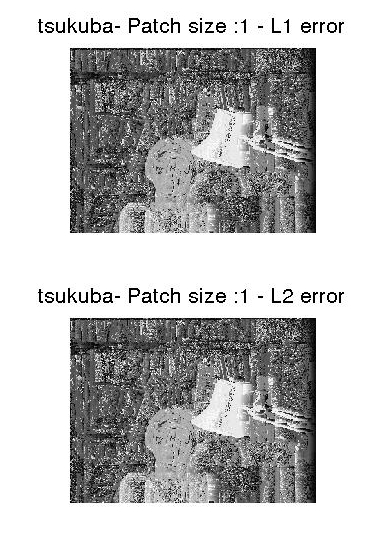
\includegraphics[scale=0.3]{./pics/tsukuba_disparity_patchsize_1.jpg}
\caption{Patch size 1}
\end{subfigure}
 \begin{subfigure}{0.5\textwidth}
 \centering
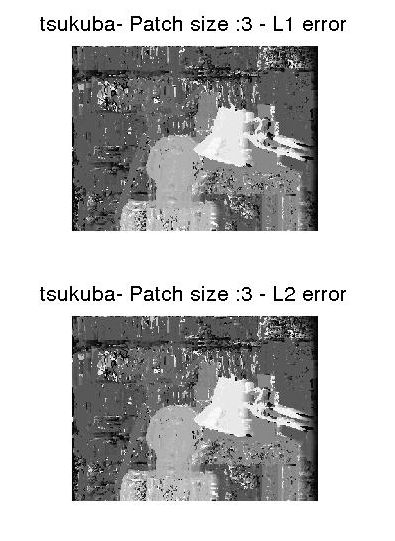
\includegraphics[scale=0.3]{./pics/tsukuba_disparity_patchsize_3.jpg}
\caption{Patch size 3}
\end{subfigure}
 \begin{subfigure}{0.5\textwidth}
 \centering
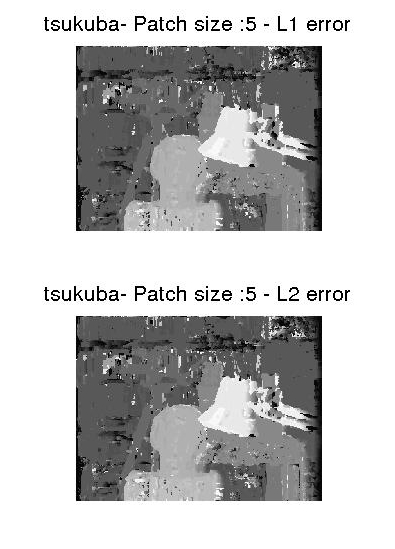
\includegraphics[scale=0.3]{./pics/tsukuba_disparity_patchsize_5.jpg}
\caption{Patch size 5}
\end{subfigure}
 \begin{subfigure}{0.5\textwidth}
 \centering
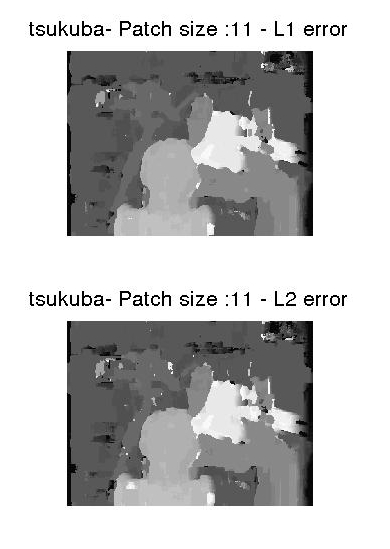
\includegraphics[scale=0.3]{./pics/tsukuba_disparity_patchsize_11.jpg}
\caption{Patch size 11}
\end{subfigure}
 \begin{subfigure}{0.5\textwidth}
 \centering
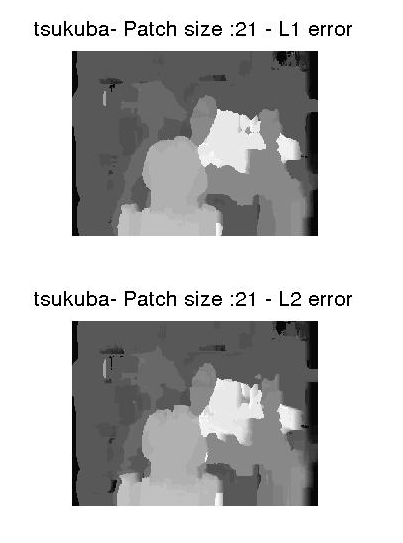
\includegraphics[scale=0.3]{./pics/tsukuba_disparity_patchsize_21.jpg}
\caption{Patch size 21}
\end{subfigure}
\end{figure}

\newpage
\section{Using Graph cuts}
\subsection{map (black \& white) image}
\subsubsection{L1 cost function}
\begin{figure}[!ht]
 \begin{subfigure}{0.5\textwidth}
 \centering
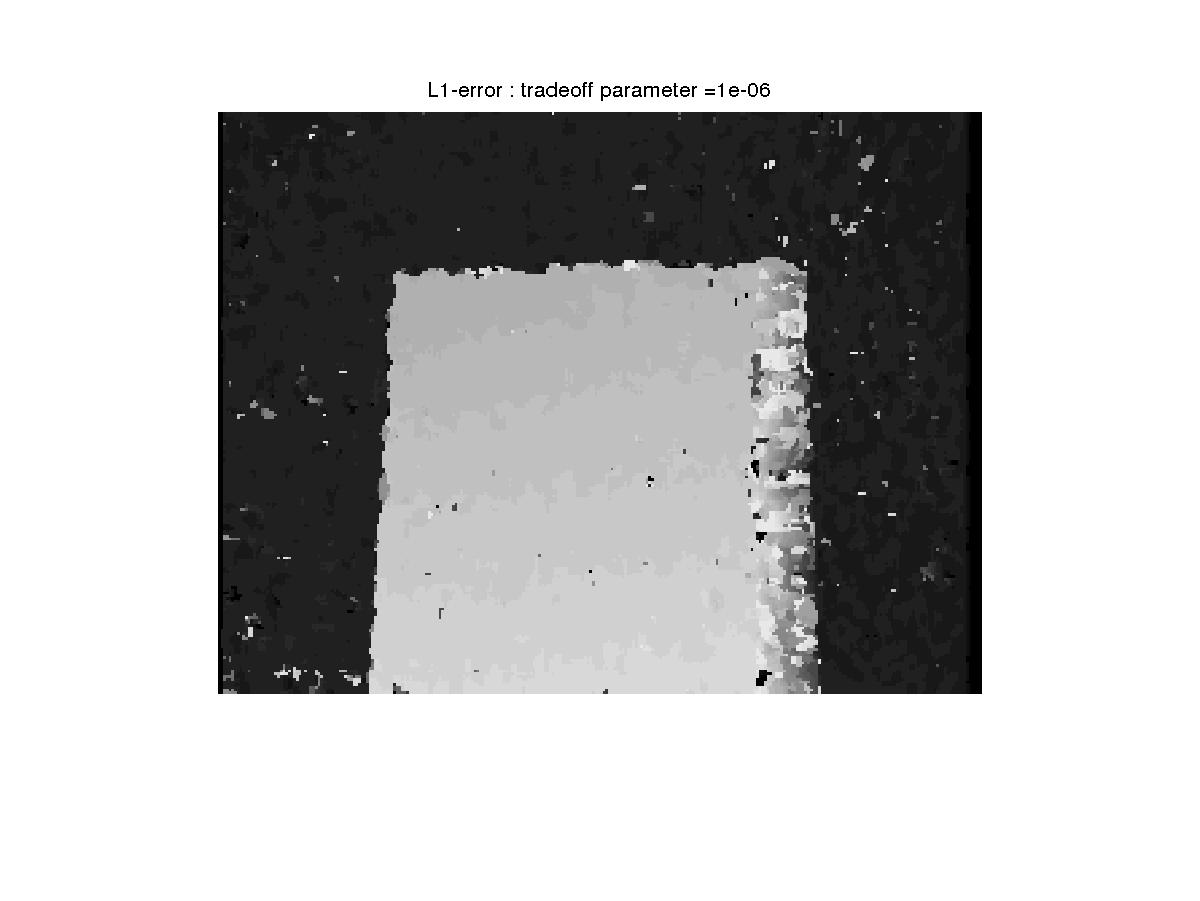
\includegraphics[scale=0.2]{./pics/map_L1_error_p=1e-06.jpg}
\caption{L1 error with p=1e-6}
\end{subfigure}
 \begin{subfigure}{0.5\textwidth}
 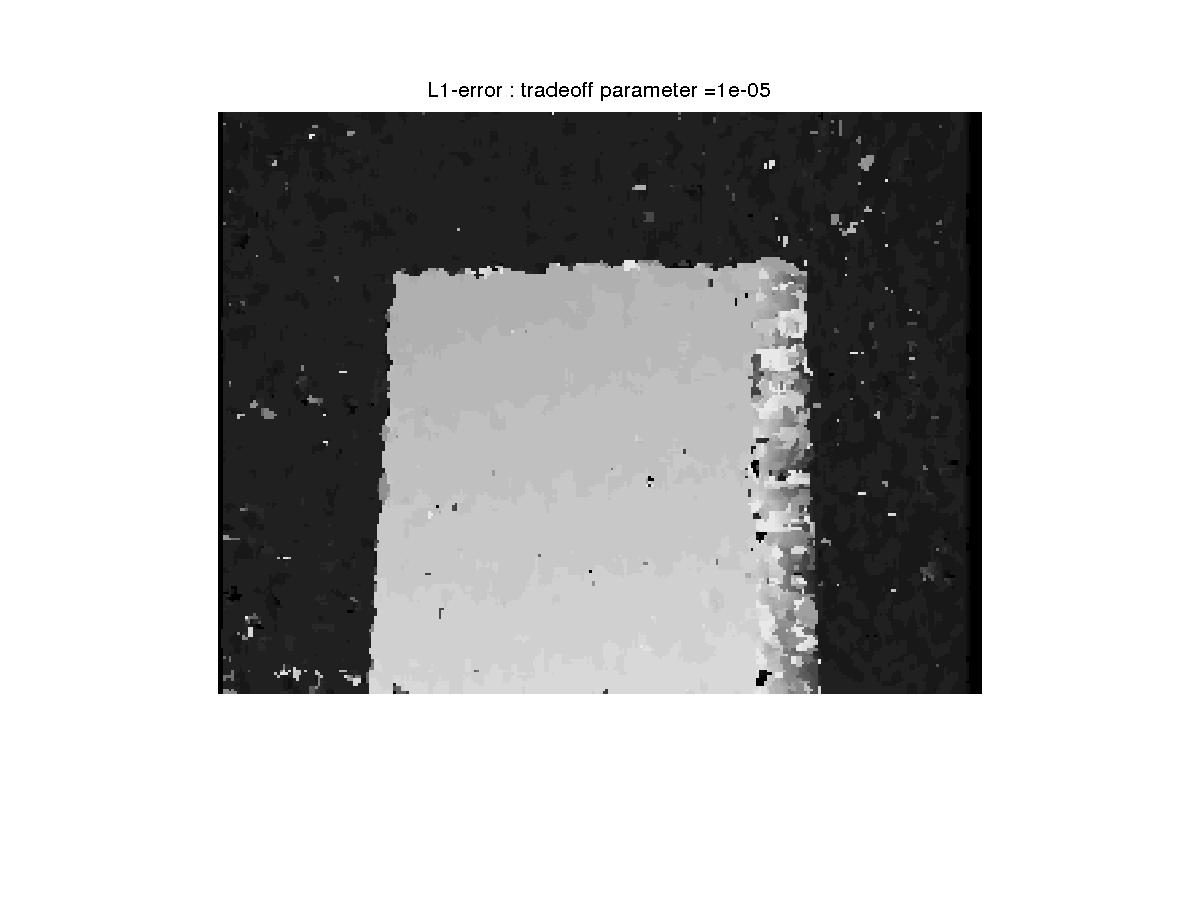
\includegraphics[scale=0.2]{./pics/map_L1_error_p=1e-05.jpg}
 \caption{L1 error with p=1e-5}
\end{subfigure}
 \begin{subfigure}{0.5\textwidth}
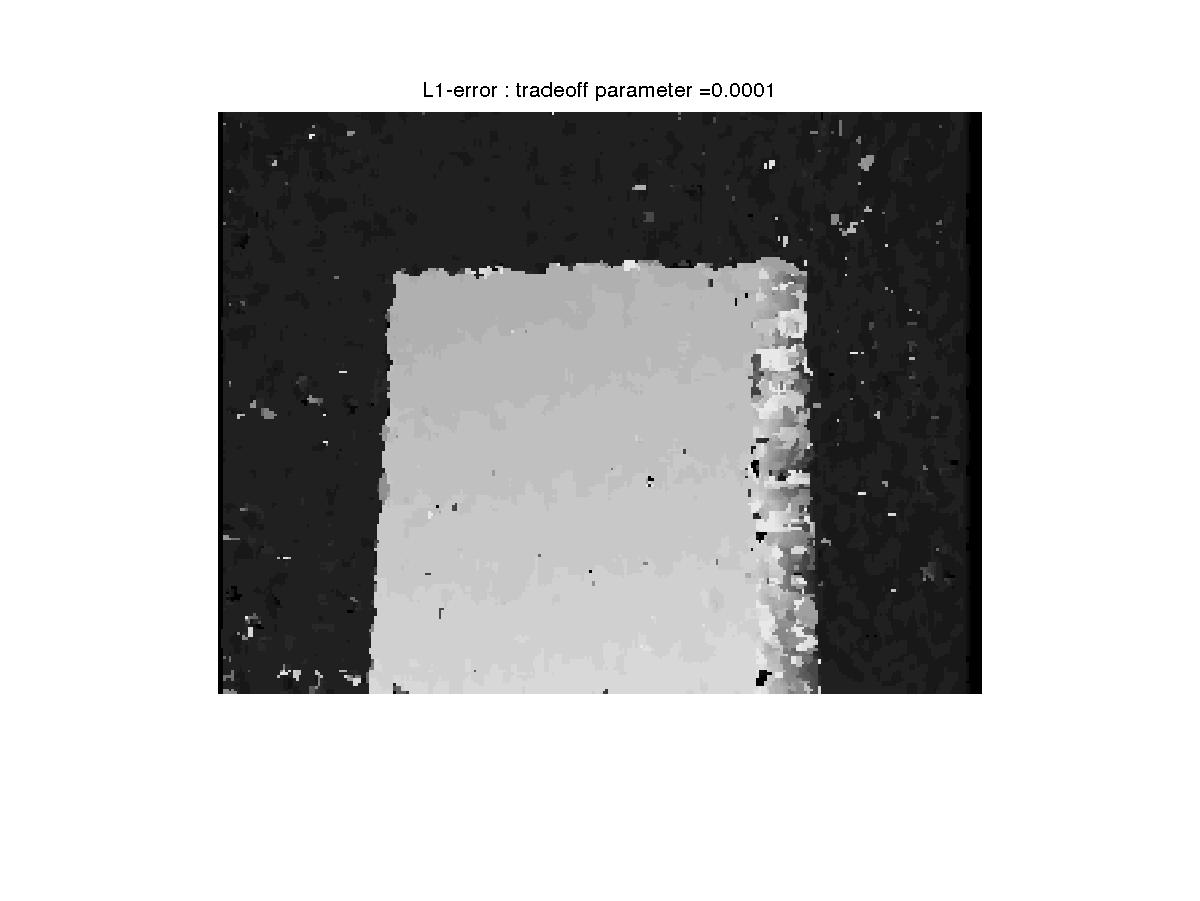
\includegraphics[scale=0.2]{./pics/map_L1_error_p=0.0001.jpg}
\caption{L1 error with p=0.0001}
\end{subfigure}
 \begin{subfigure}{0.5\textwidth}
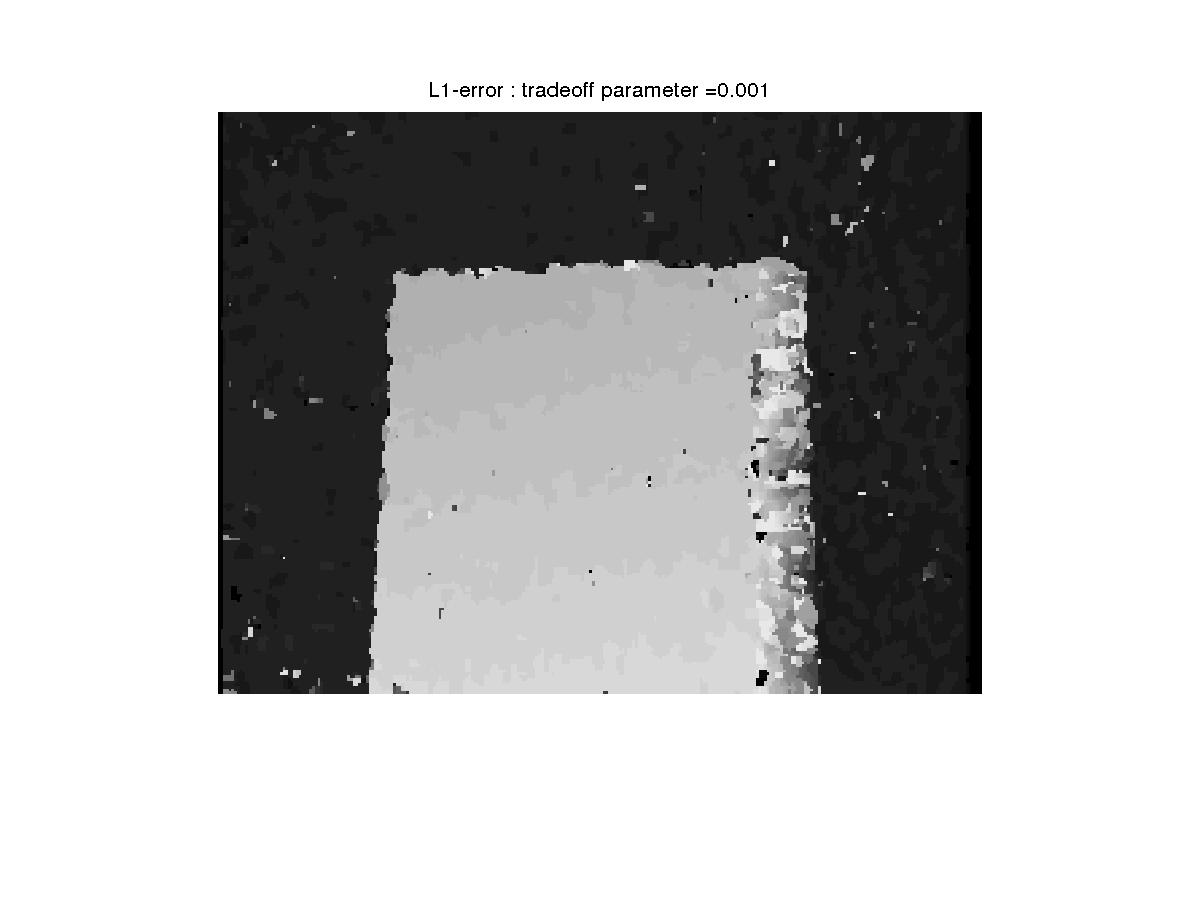
\includegraphics[scale=0.2]{./pics/map_L1_error_p=0.001.jpg}
\caption{L1 error with p=0.001}
\end{subfigure}
 \begin{subfigure}{0.5\textwidth}
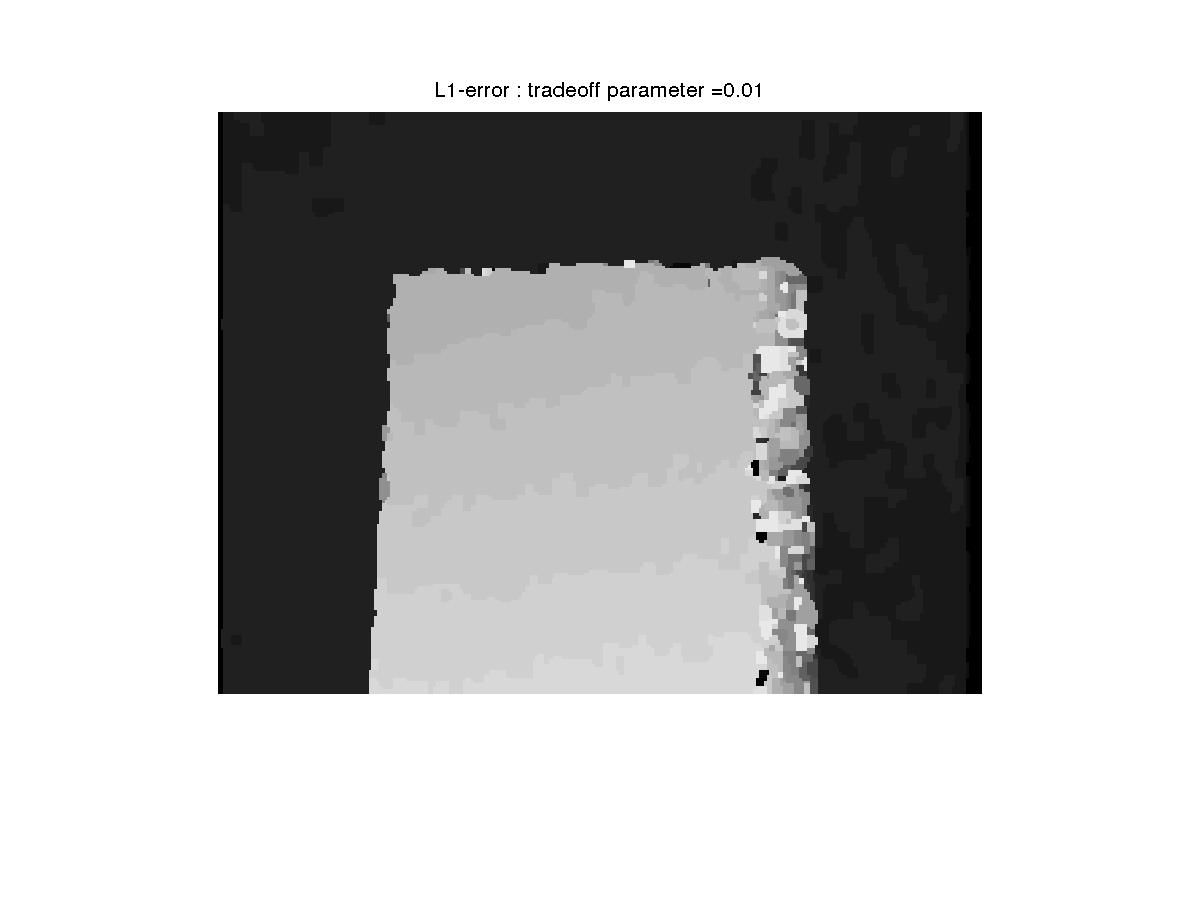
\includegraphics[scale=0.2]{./pics/map_L1_error_p=0.01.jpg}
\caption{L1 error with p=0.01}
\end{subfigure}
 \begin{subfigure}{0.5\textwidth}
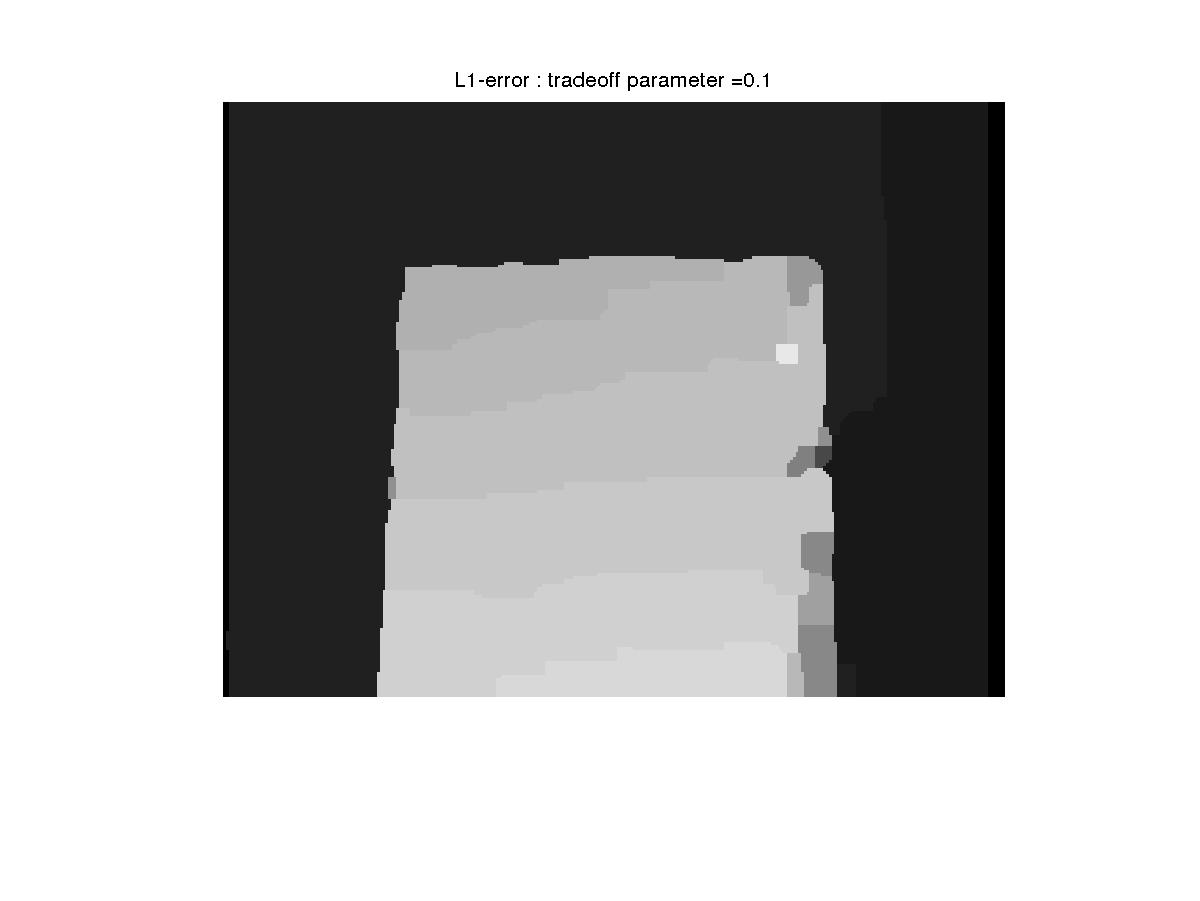
\includegraphics[scale=0.2]{./pics/map_L1_error_p=0.1.jpg}
\caption{L1 error with p=0.1}
\end{subfigure}
\end{figure}
\begin{figure}
 \begin{subfigure}{0.5\textwidth}
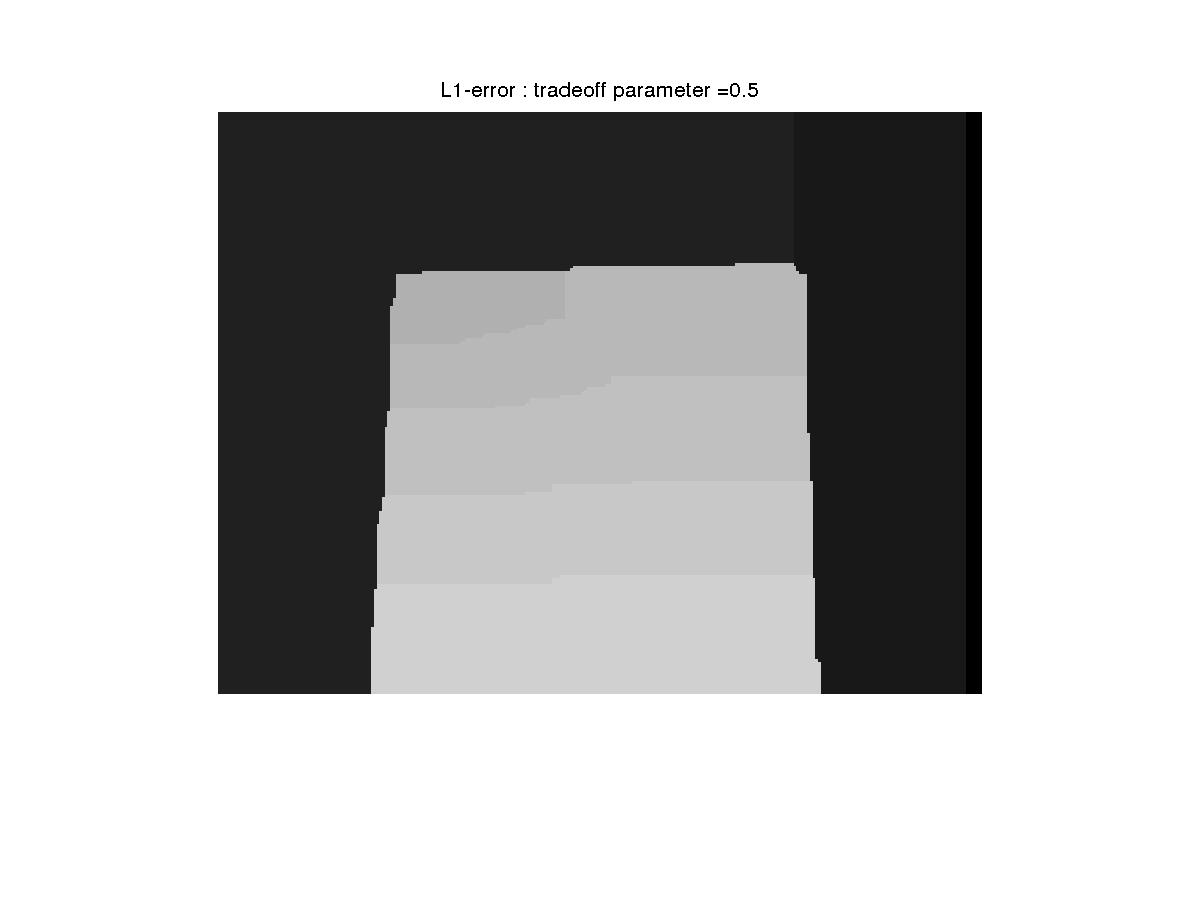
\includegraphics[scale=0.2]{./pics/map_L1_error_p=0.5.jpg}
\caption{L1 error with p=0.5}
\end{subfigure}
 \begin{subfigure}{0.5\textwidth}
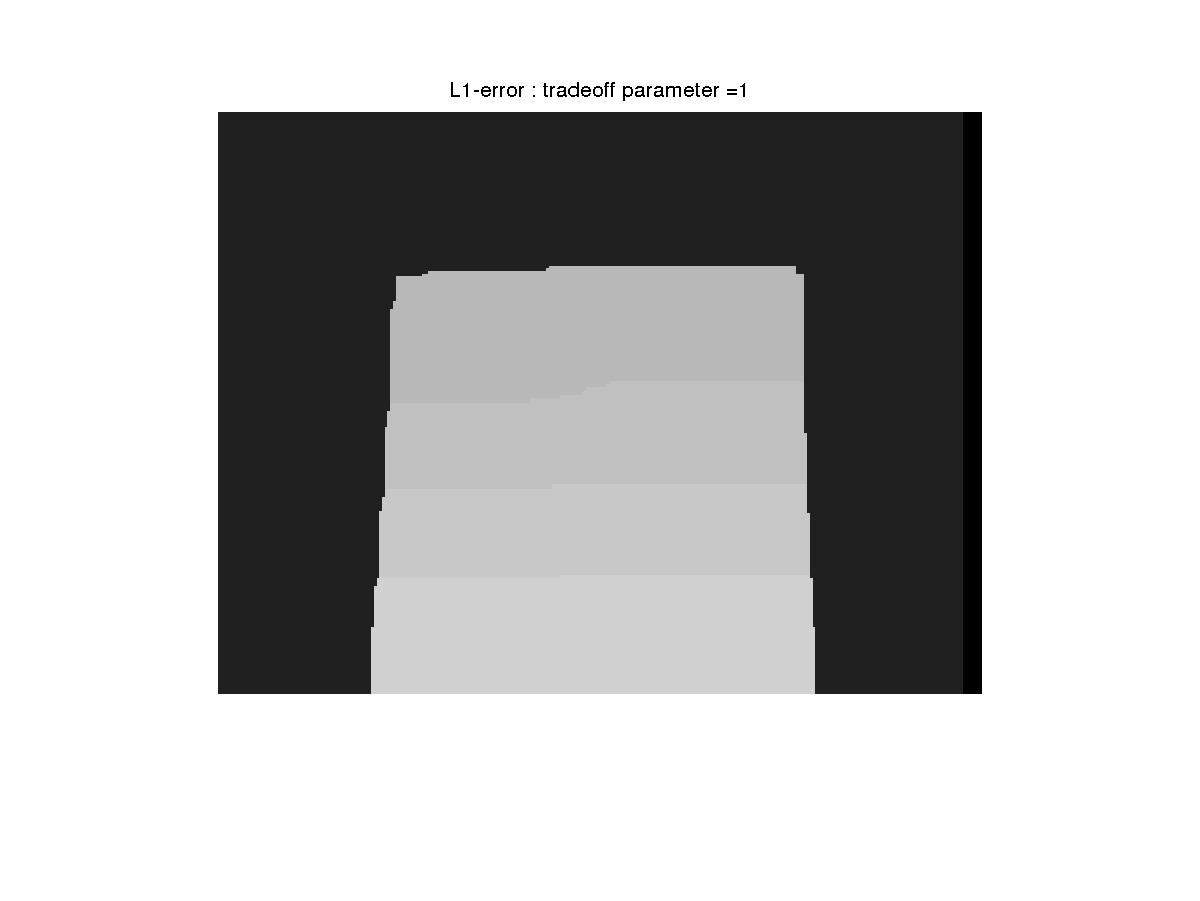
\includegraphics[scale=0.2]{./pics/map_L1_error_p=1.jpg}
\caption{L1 error with p=1}
\end{subfigure}
 \begin{subfigure}{0.5\textwidth}
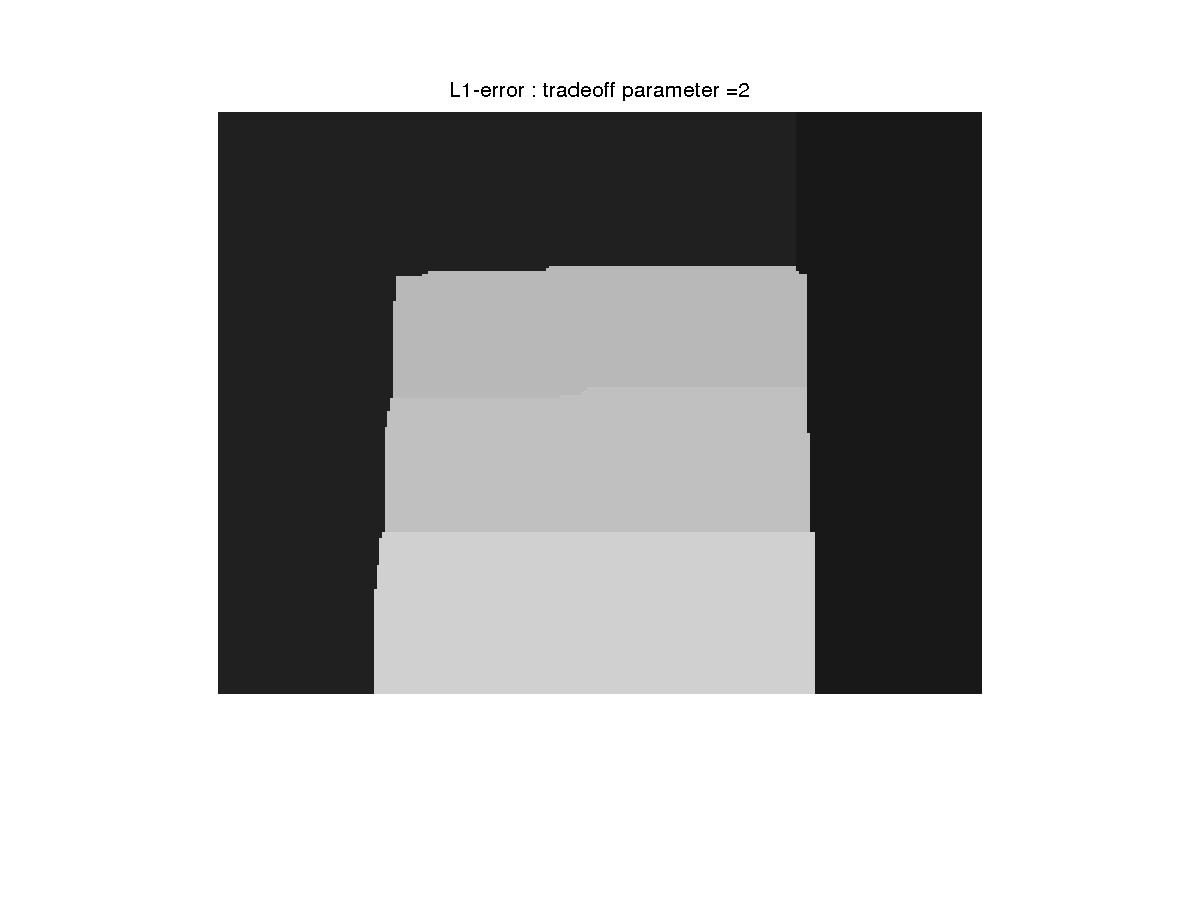
\includegraphics[scale=0.2]{./pics/map_L1_error_p=2.jpg}
\caption{L1 error with p=2}
\end{subfigure}
 \begin{subfigure}{0.5\textwidth}
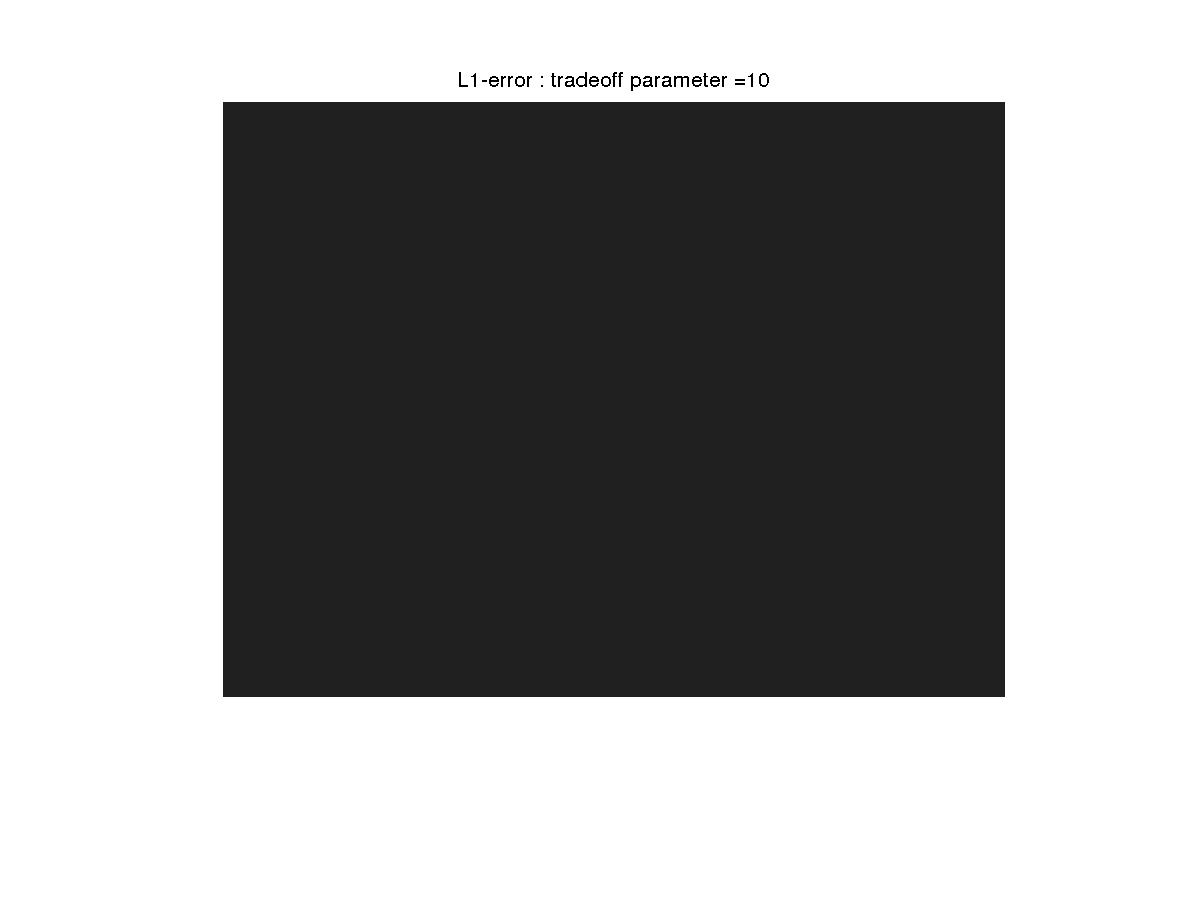
\includegraphics[scale=0.2]{./pics/map_L1_error_p=10.jpg}
\caption{L1 error with p=10}
\end{subfigure}
\end{figure}
As we can see in the figures, when the trade-off parameter (p) is higher (=10), 
the smoothness is given more weightage and the whole image is turned into a constant color.
The best value for p is 0.1.

\subsubsection{L2 cost function}
\begin{figure}[!ht]
 \begin{subfigure}{0.5\textwidth}
 \centering
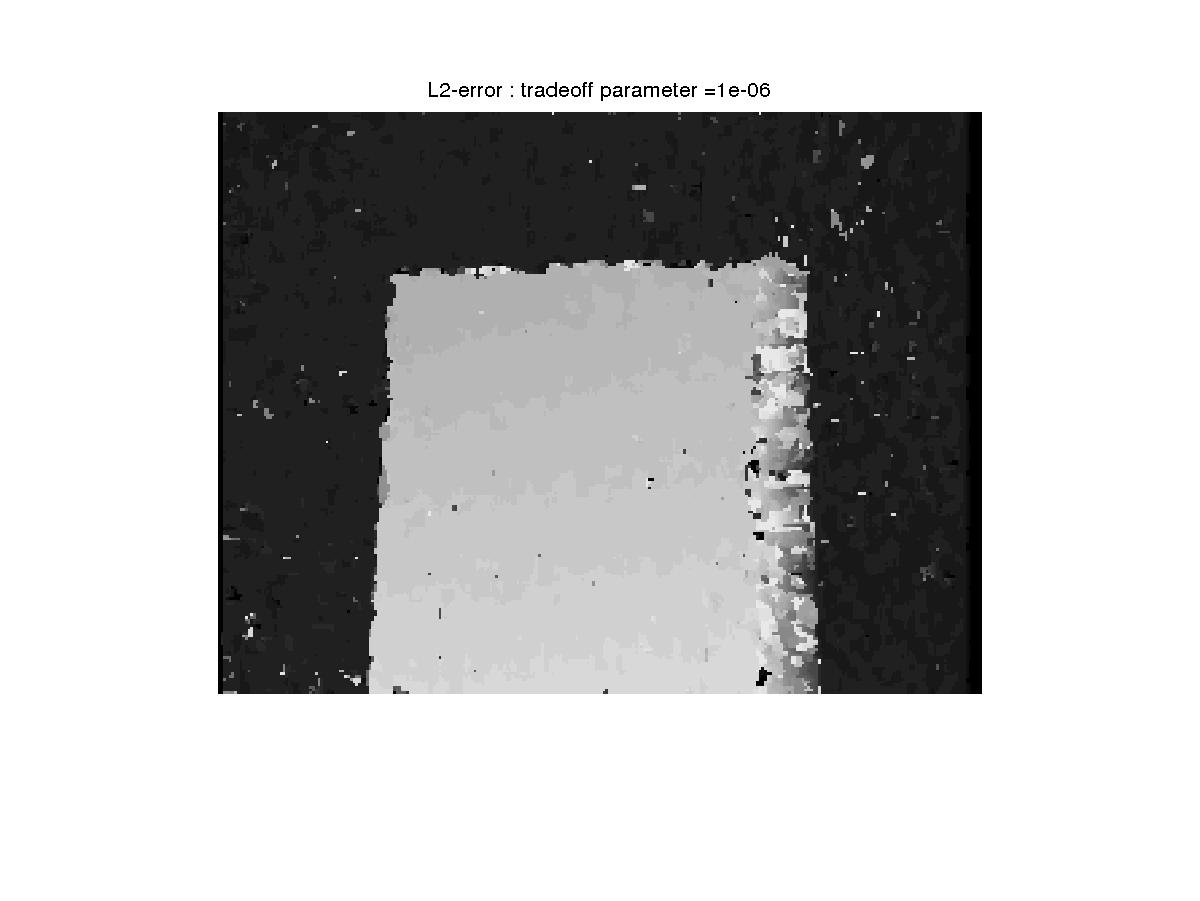
\includegraphics[scale=0.2]{./pics/map_L2_error_p=1e-06.jpg}
\caption{L2 error with p=1e-6}
\end{subfigure}
 \begin{subfigure}{0.5\textwidth}
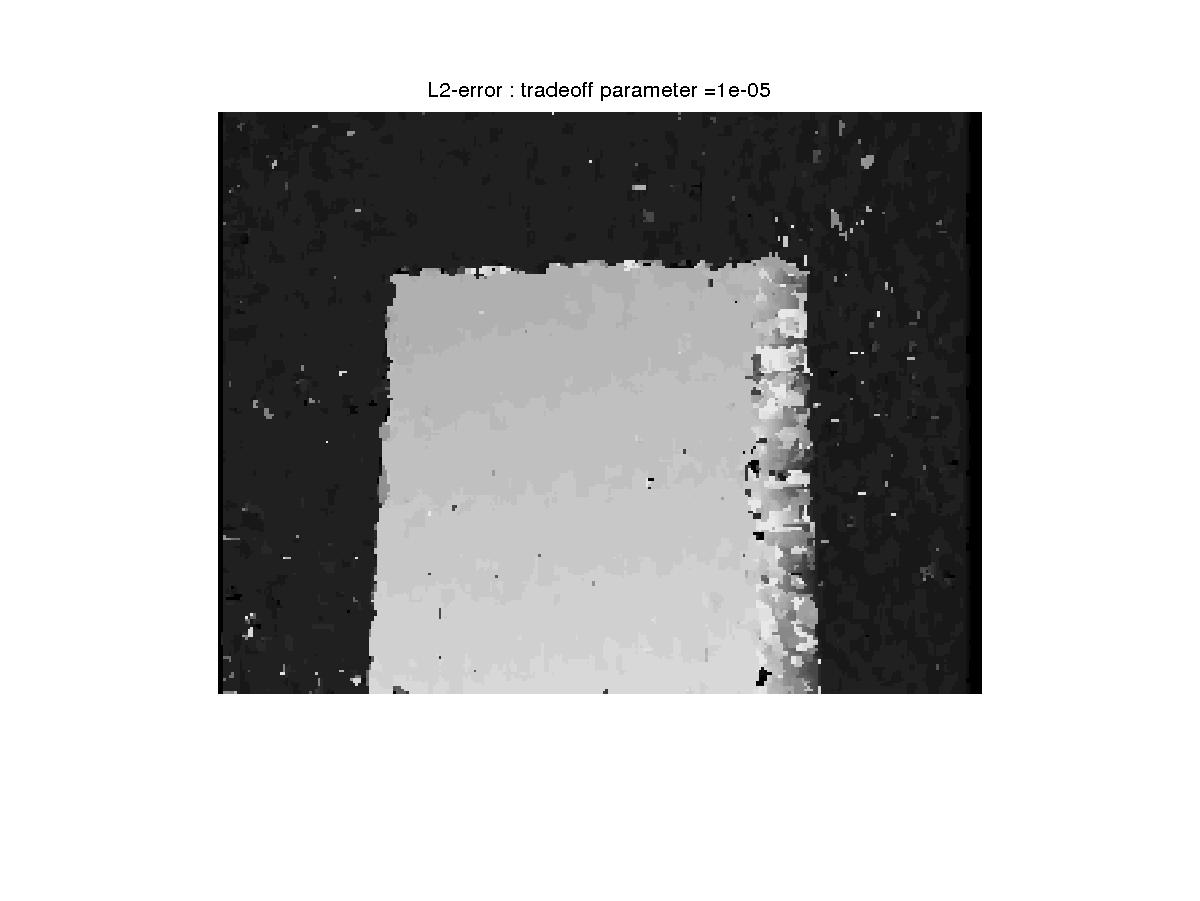
\includegraphics[scale=0.2]{./pics/map_L2_error_p=1e-05.jpg}
\caption{L2 error with p=1e-5}
\end{subfigure}
 \begin{subfigure}{0.5\textwidth}
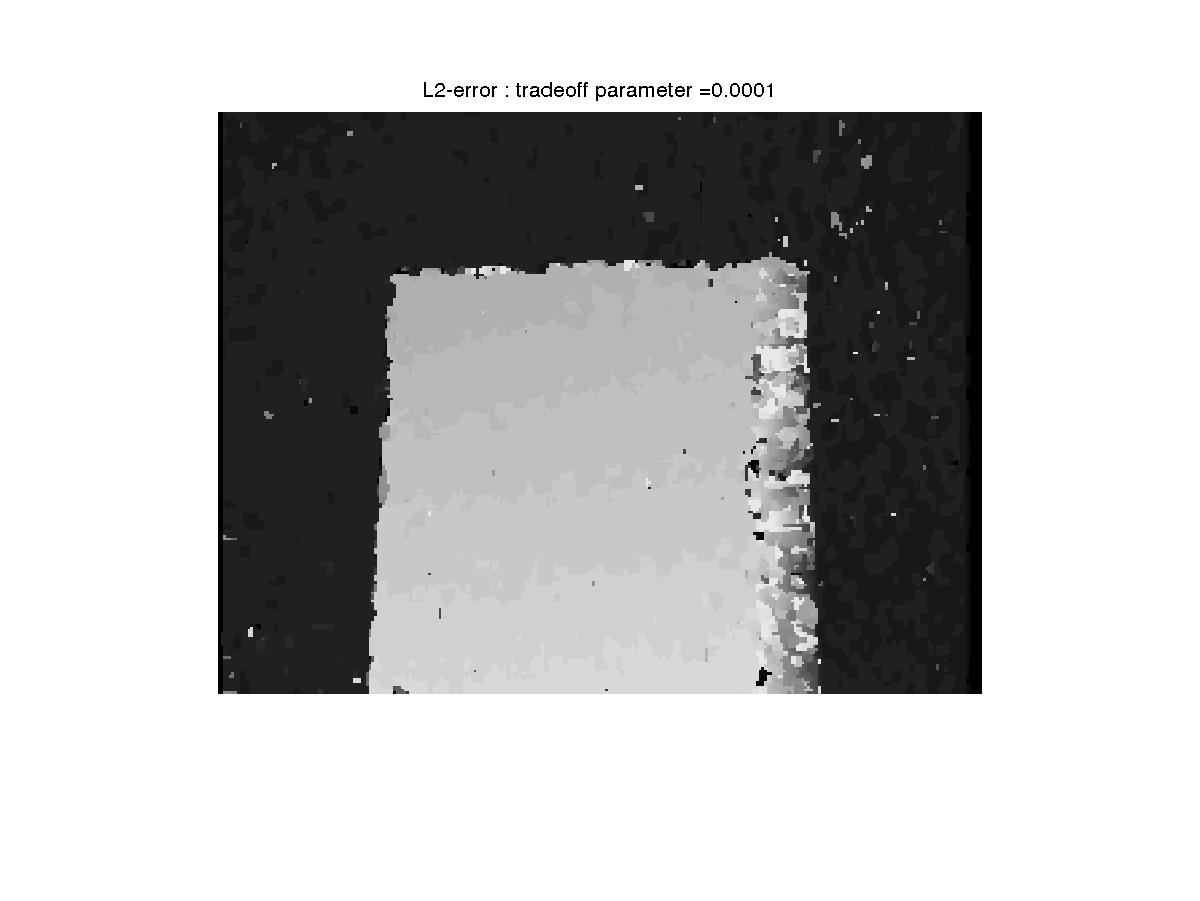
\includegraphics[scale=0.2]{./pics/map_L2_error_p=0.0001.jpg}
\caption{L2 error with p=0.0001}
\end{subfigure}
 \begin{subfigure}{0.5\textwidth}
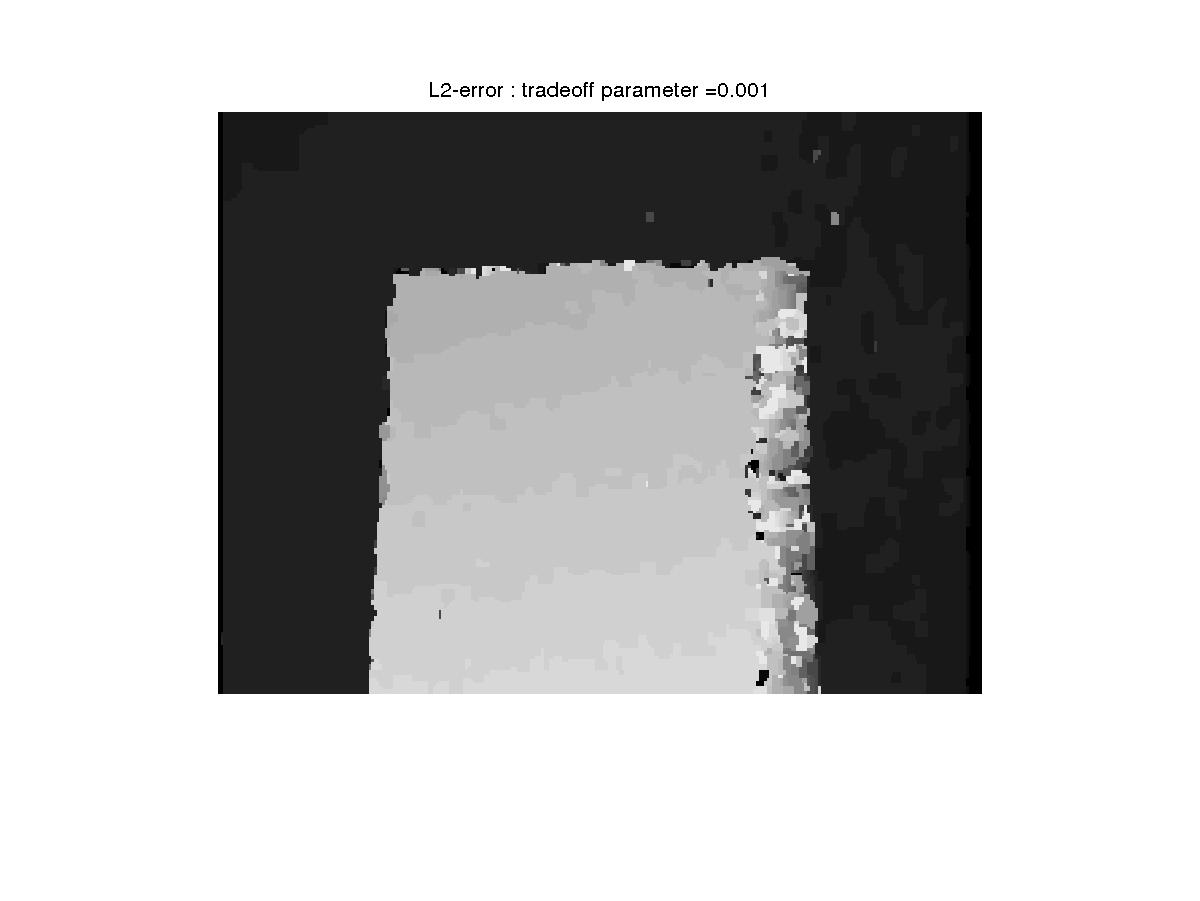
\includegraphics[scale=0.2]{./pics/map_L2_error_p=0.001.jpg}
\caption{L2 error with p=0.001}
\end{subfigure}
 \begin{subfigure}{0.5\textwidth}
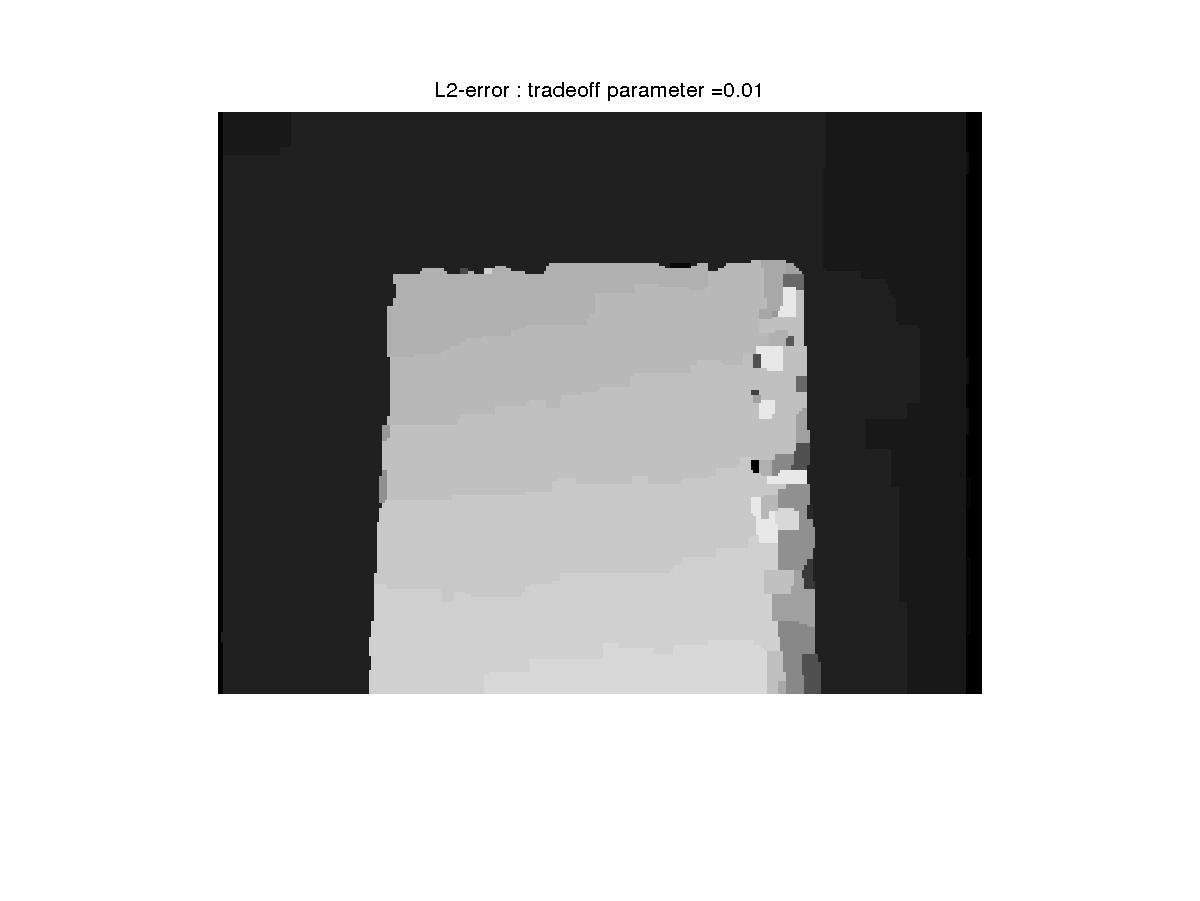
\includegraphics[scale=0.2]{./pics/map_L2_error_p=0.01.jpg}
\caption{L2 error with p=0.01}
\end{subfigure}
 \begin{subfigure}{0.5\textwidth}
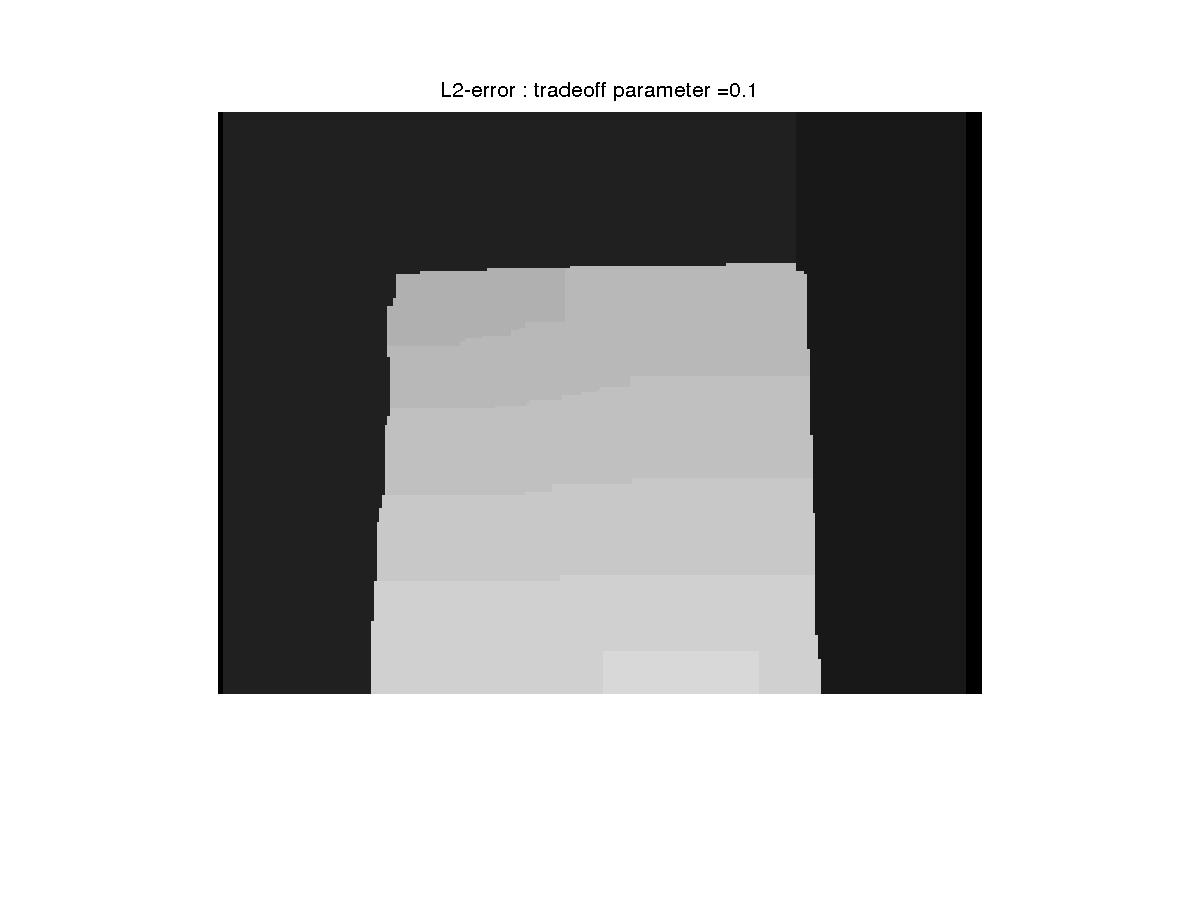
\includegraphics[scale=0.2]{./pics/map_L2_error_p=0.1.jpg}
\caption{L2 error with p=0.1}
\end{subfigure}
\end{figure}
\begin{figure}
 \begin{subfigure}{0.5\textwidth}
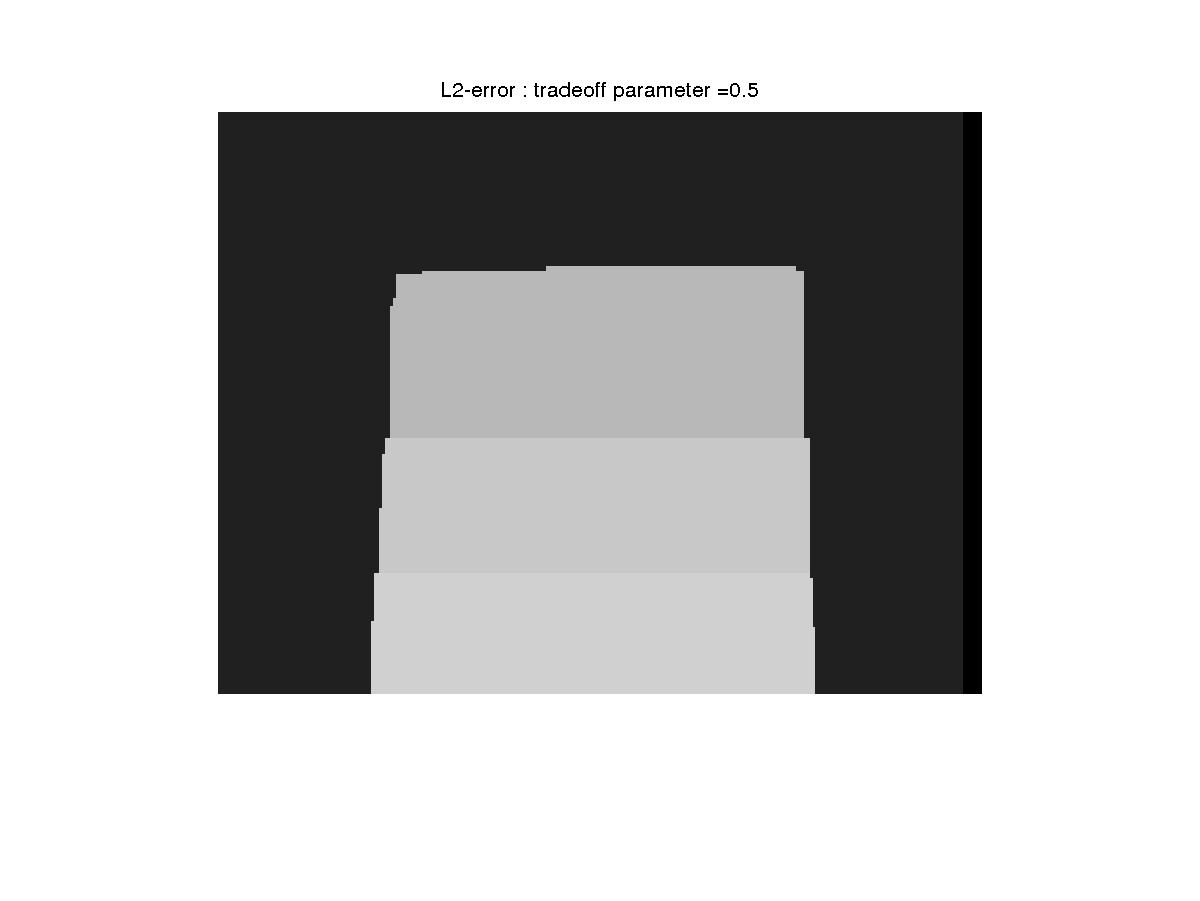
\includegraphics[scale=0.2]{./pics/map_L2_error_p=0.5.jpg}
\caption{L2 error with p=0.5}
\end{subfigure}
 \begin{subfigure}{0.5\textwidth}
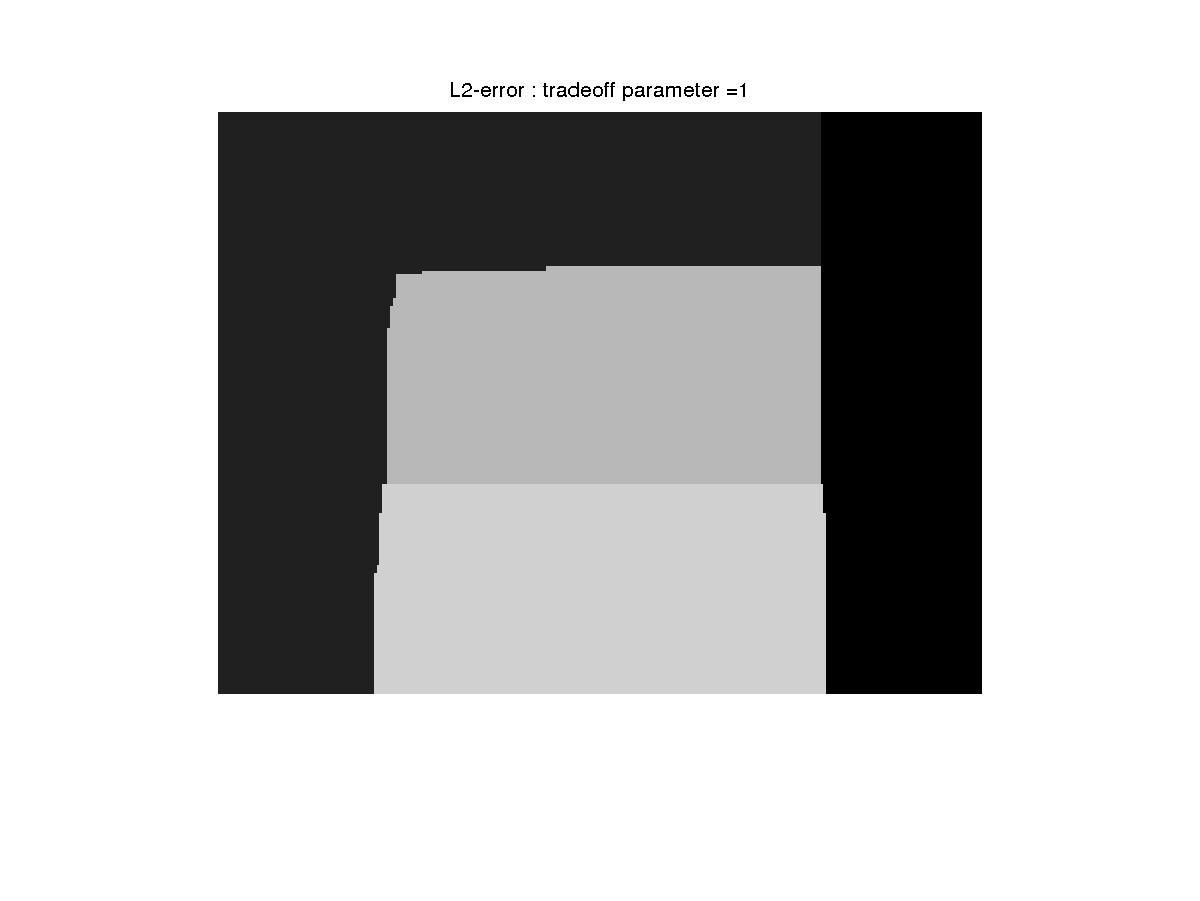
\includegraphics[scale=0.2]{./pics/map_L2_error_p=1.jpg}
\caption{L2 error with p=1}
\end{subfigure}
 \begin{subfigure}{0.5\textwidth}
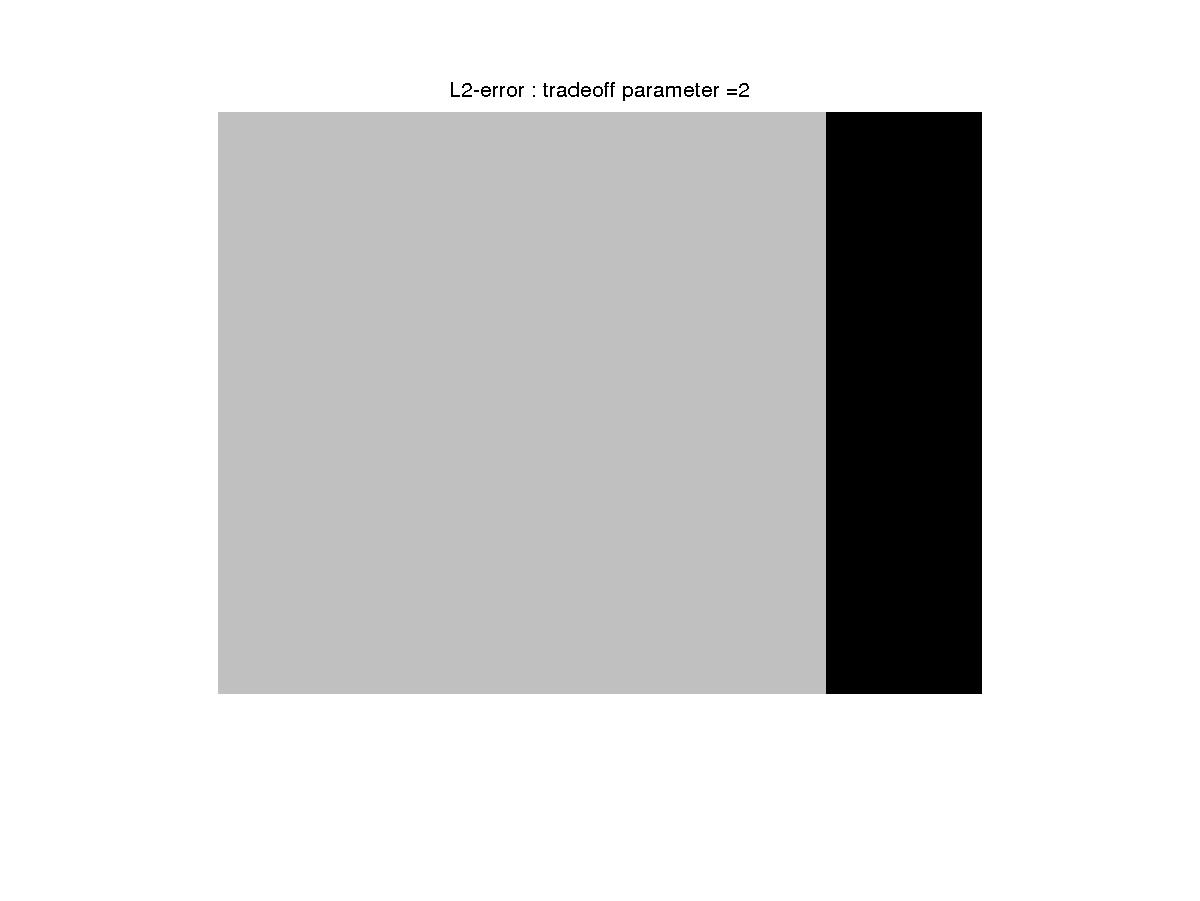
\includegraphics[scale=0.2]{./pics/map_L2_error_p=2.jpg}
\caption{L2 error with p=2}
\end{subfigure}
 \begin{subfigure}{0.5\textwidth}
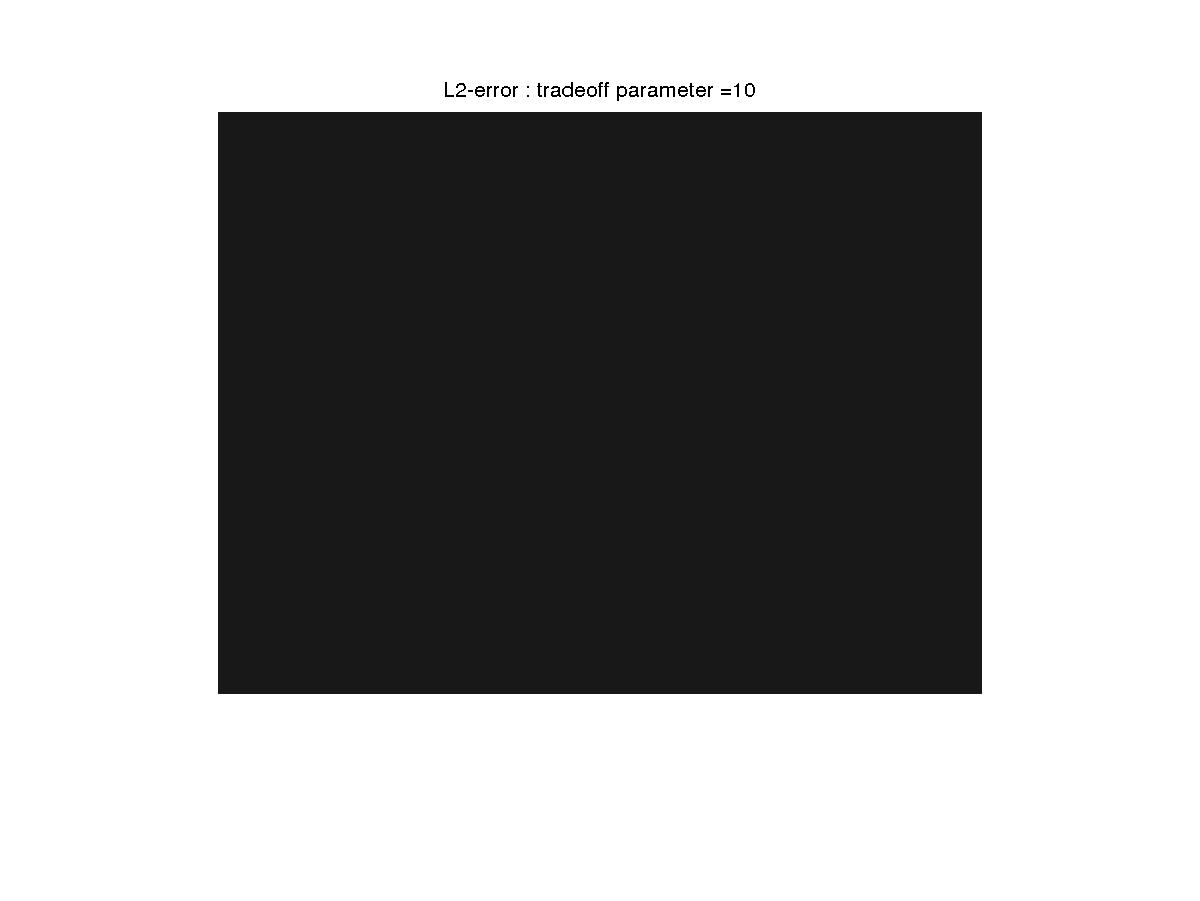
\includegraphics[scale=0.2]{./pics/map_L2_error_p=10.jpg}
\caption{L2 error with p=10}
\end{subfigure}
\end{figure}

As we can see in the figure, when the trade-off parameter (p) is higher (=10), 
the smoothness is given more weightage and the whole image is turned into a constant.
The best value for p is 0.01.

\subsubsection{Error vs. Trade-off parameter(p)}
 \begin{figure}[!ht]
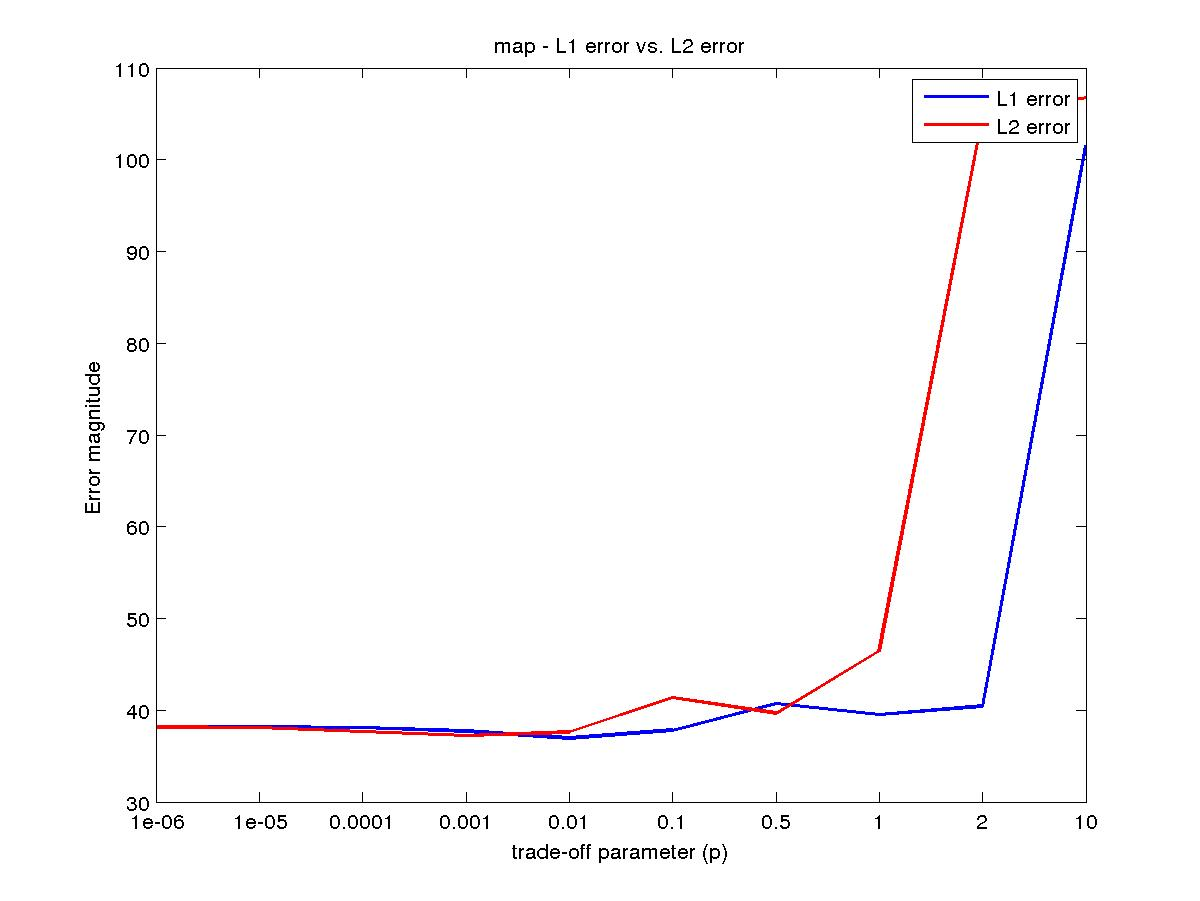
\includegraphics[scale=0.3]{./pics/_error_vs_tradeoffparams.jpg}
\caption{As per the observation, p=0.1 for L1 error, p=0.01 for L2 error are the best trade-off parameter}
\end{figure}

\clearpage
\subsection{tsukuba image}
\subsubsection{L1 cost function}
\begin{figure}[!ht]
 \begin{subfigure}{0.5\textwidth}
 \centering
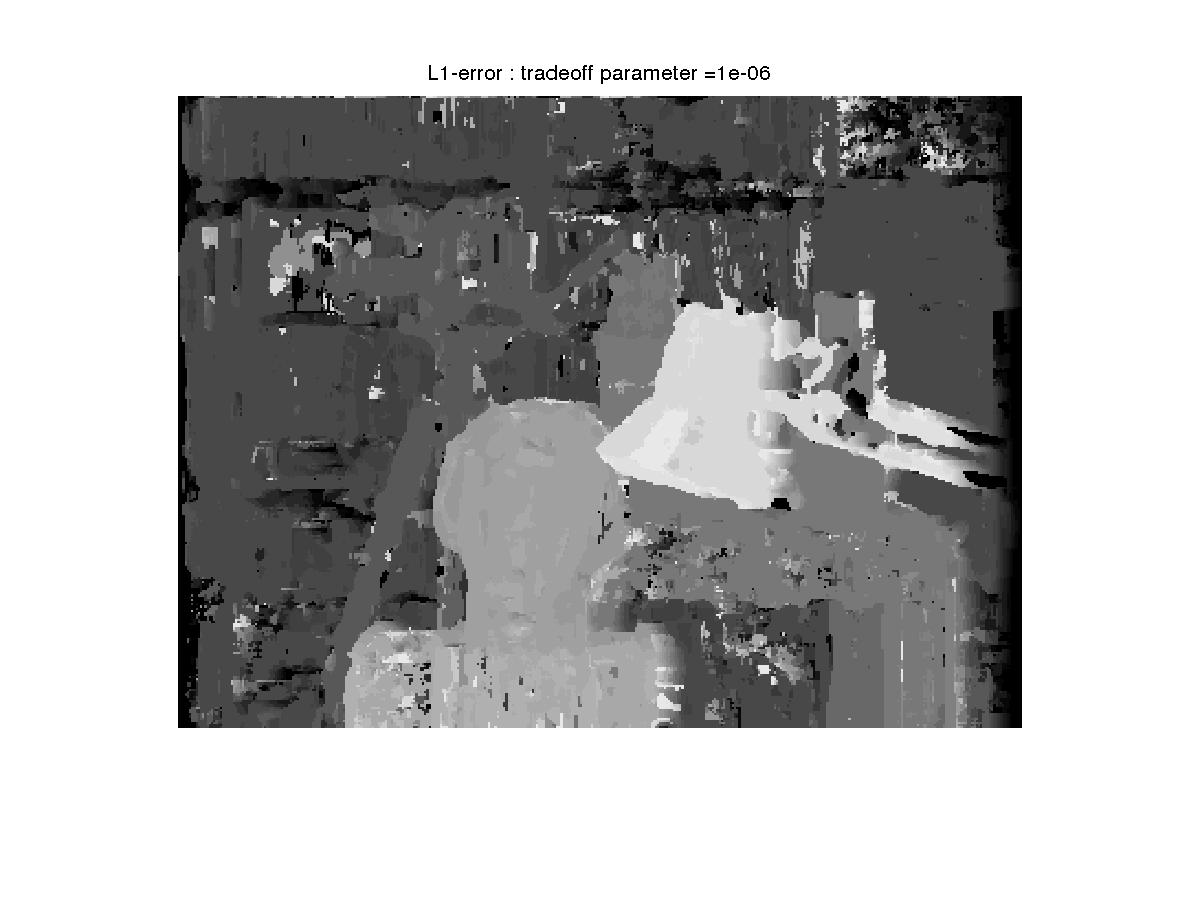
\includegraphics[scale=0.2]{./pics/tsukuba_L1_error_p=1e-06.jpg}
\caption{L1 error with p=1e-6}
\end{subfigure}
 \begin{subfigure}{0.5\textwidth}
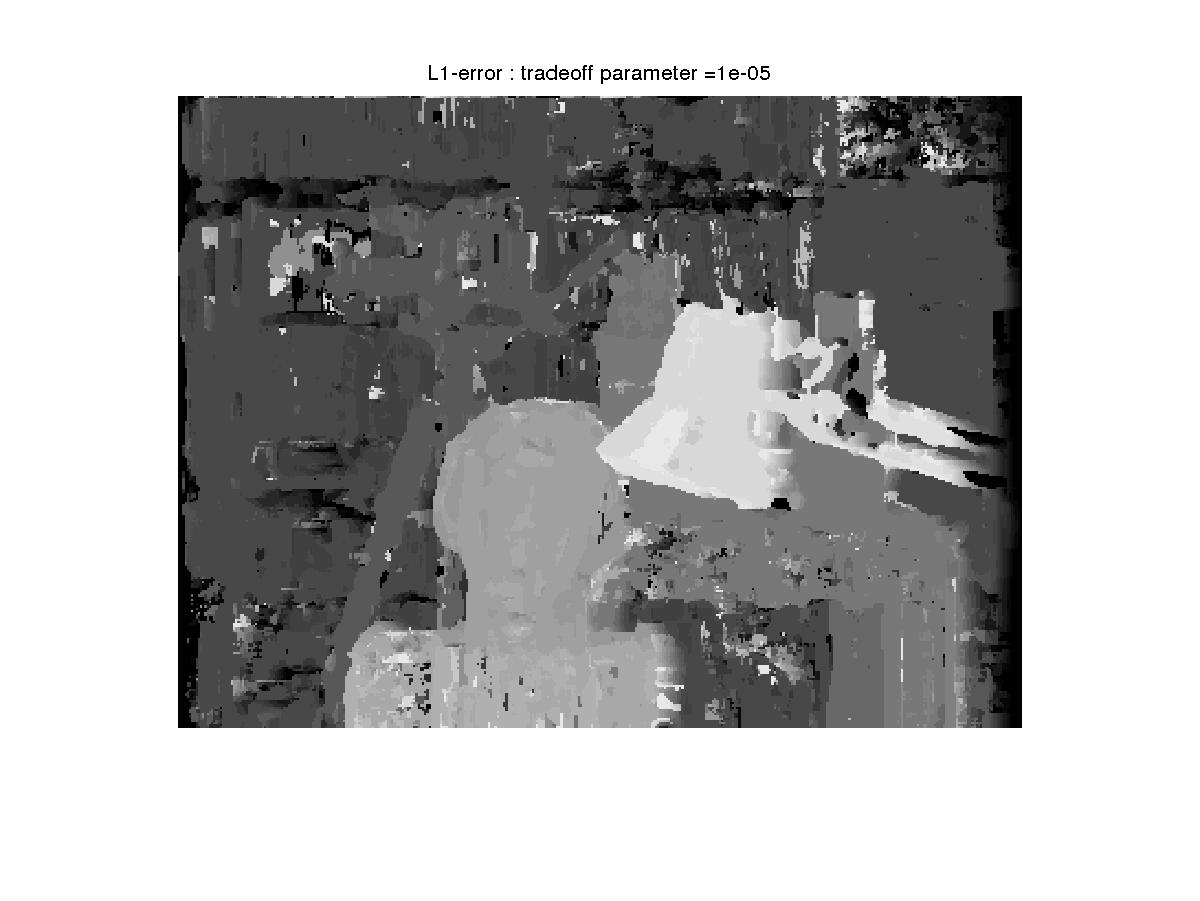
\includegraphics[scale=0.2]{./pics/tsukuba_L1_error_p=1e-05.jpg}
\caption{L1 error with p=1e-5}
\end{subfigure}
 \begin{subfigure}{0.5\textwidth}
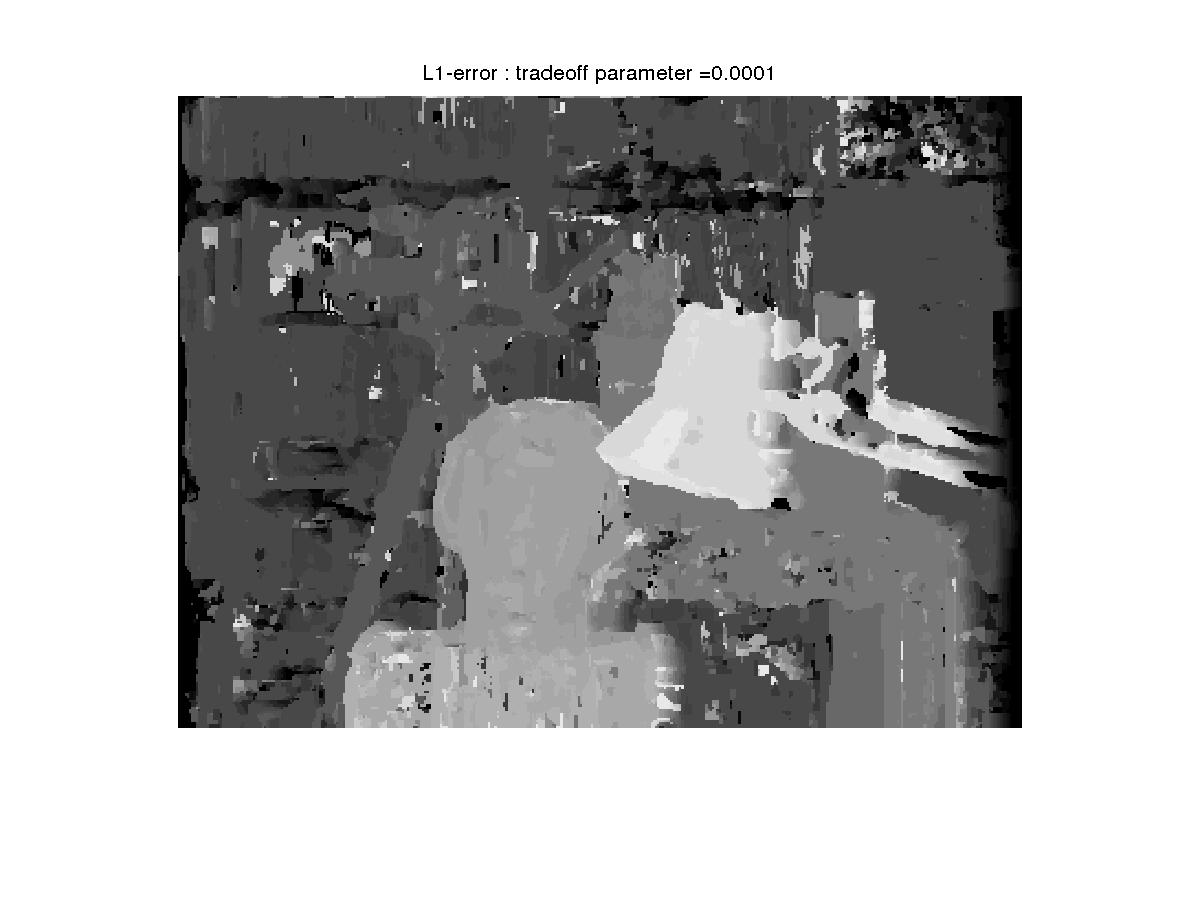
\includegraphics[scale=0.2]{./pics/tsukuba_L1_error_p=0.0001.jpg}
\caption{L1 error with p=0.0001}
\end{subfigure}
 \begin{subfigure}{0.5\textwidth}
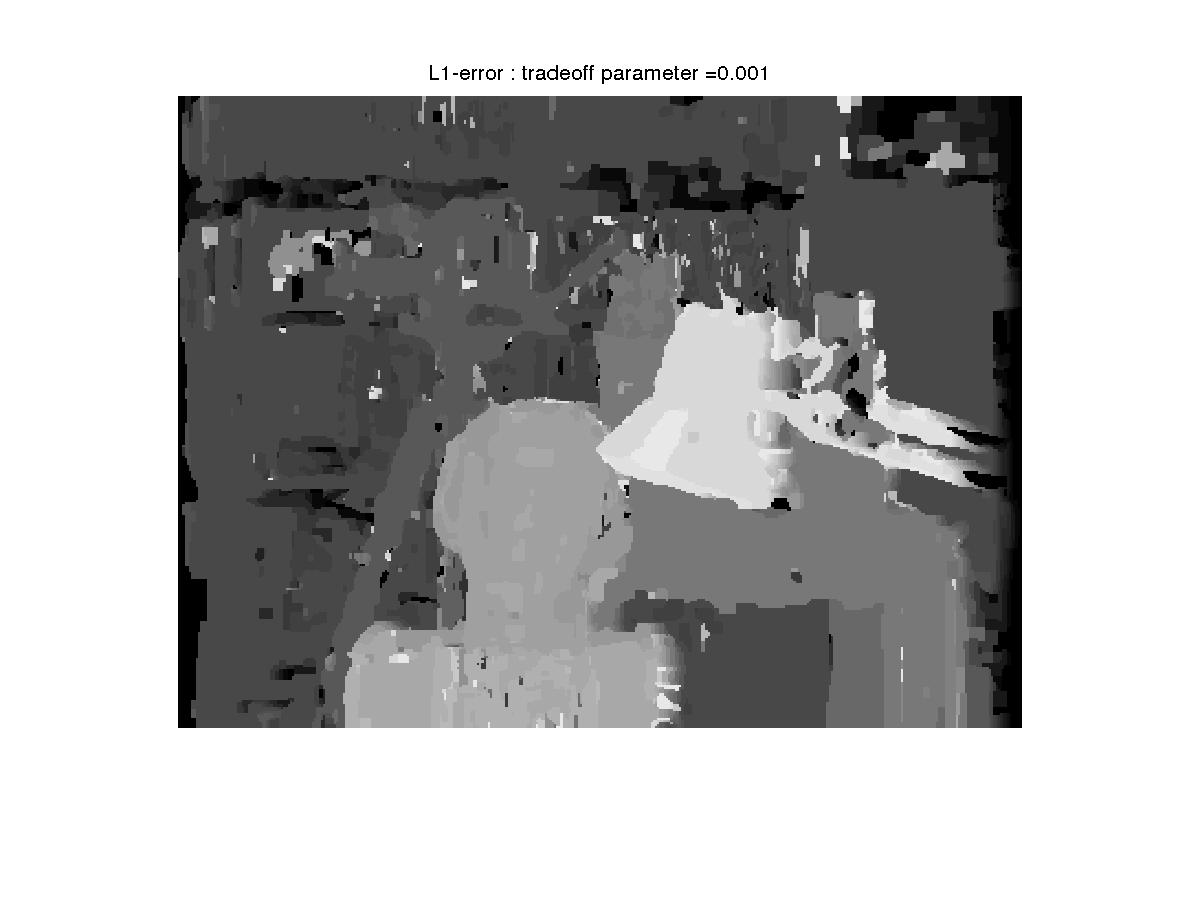
\includegraphics[scale=0.2]{./pics/tsukuba_L1_error_p=0.001.jpg}
\caption{L1 error with p=0.001}
\end{subfigure}
 \begin{subfigure}{0.5\textwidth}
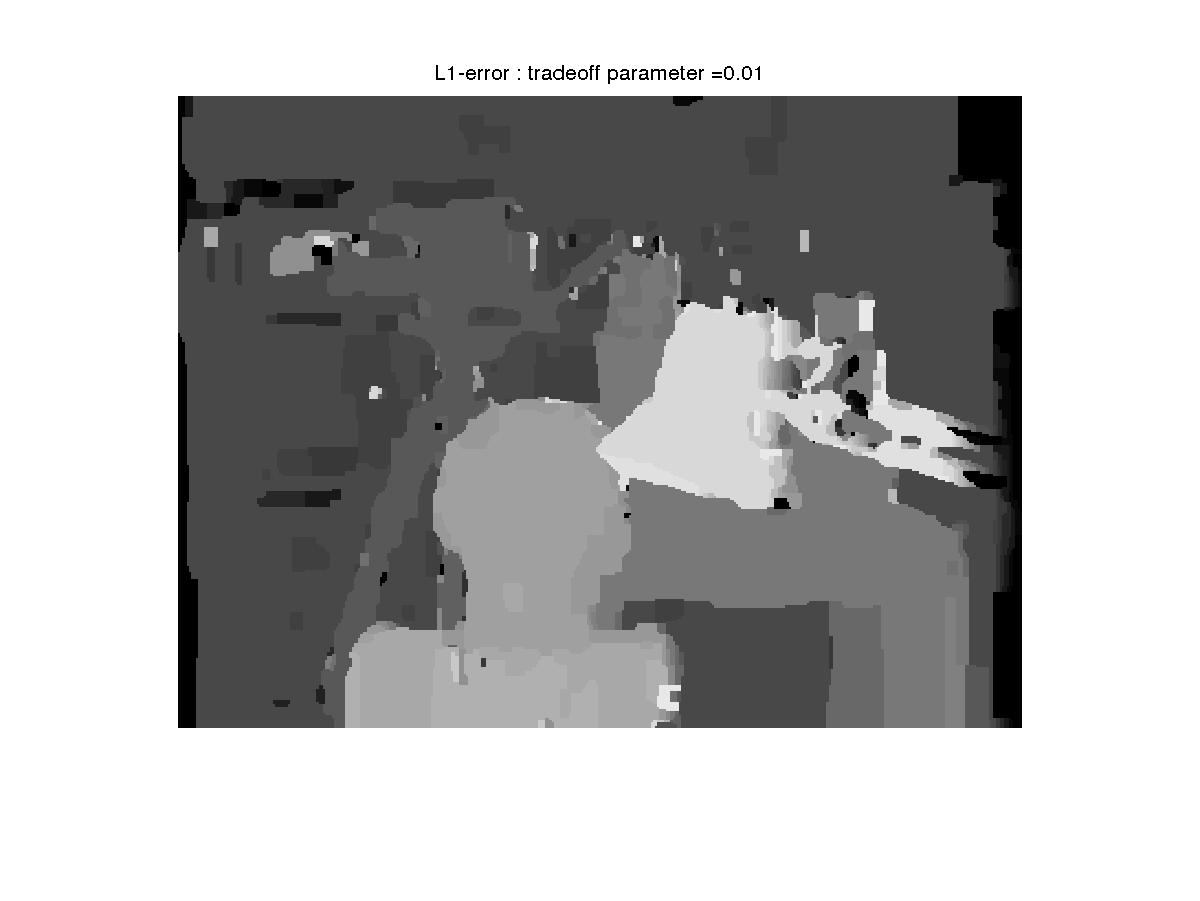
\includegraphics[scale=0.2]{./pics/tsukuba_L1_error_p=0.01.jpg}
\caption{L1 error with p=0.01}
\end{subfigure}
 \begin{subfigure}{0.5\textwidth}
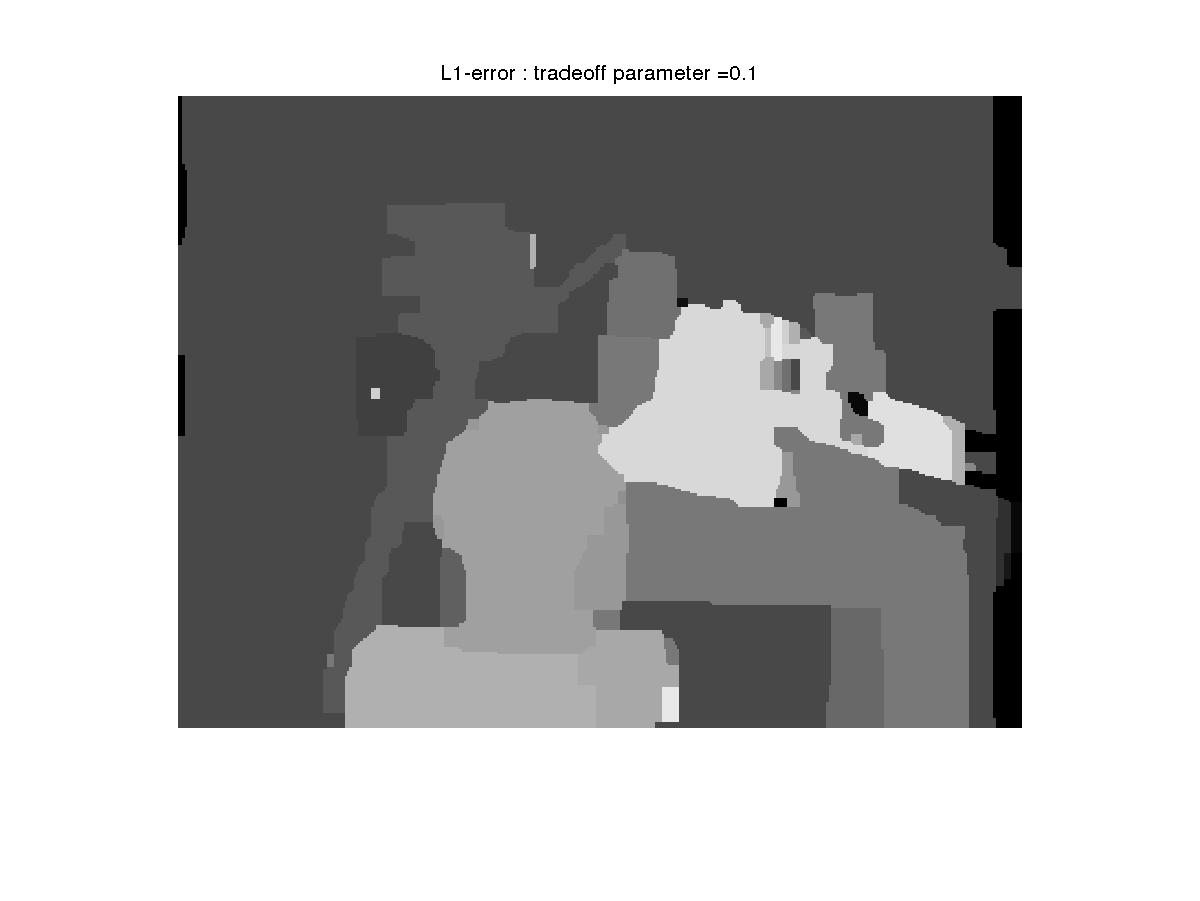
\includegraphics[scale=0.2]{./pics/tsukuba_L1_error_p=0.1.jpg}
\caption{L1 error with p=0.1}
\end{subfigure}
\end{figure}
\begin{figure}
 \begin{subfigure}{0.5\textwidth}
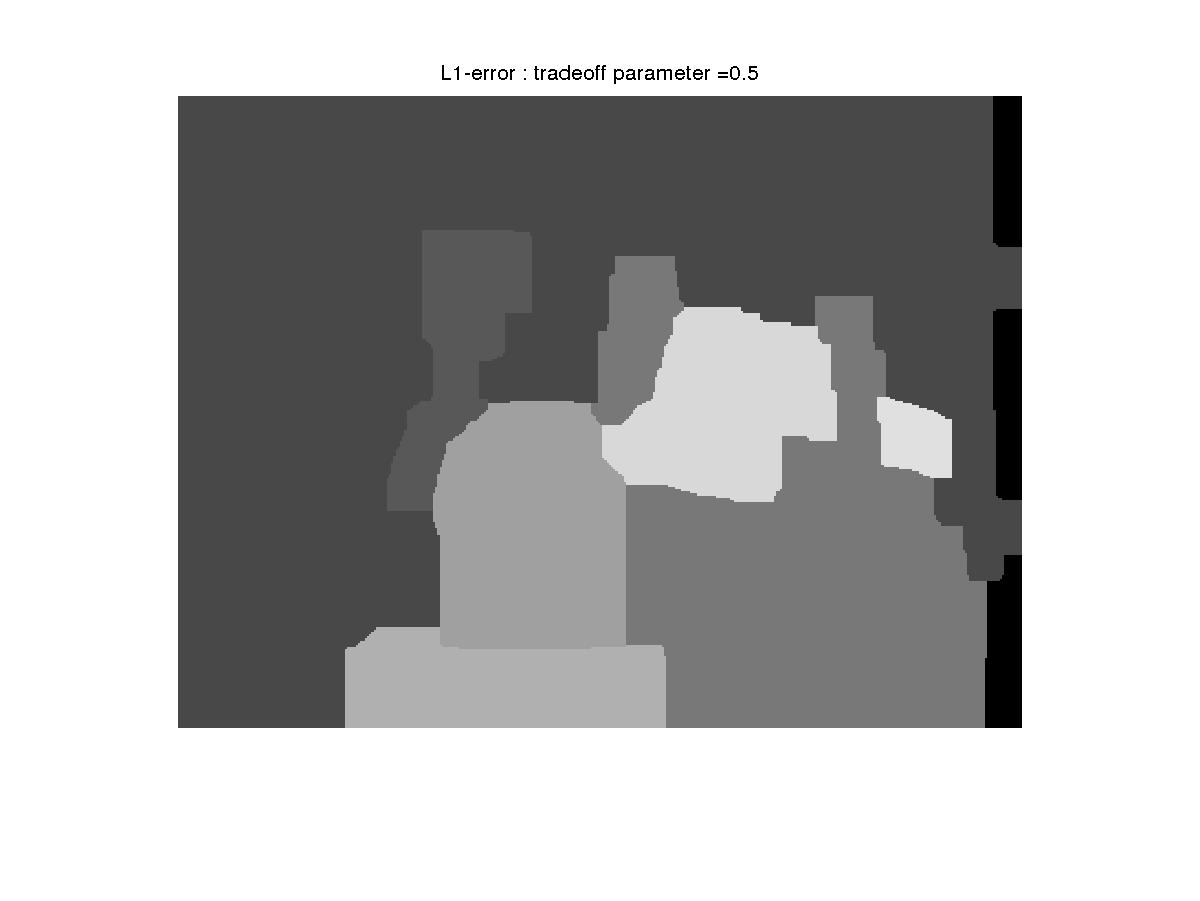
\includegraphics[scale=0.2]{./pics/tsukuba_L1_error_p=0.5.jpg}
\caption{L1 error with p=0.5}
\end{subfigure}
 \begin{subfigure}{0.5\textwidth}
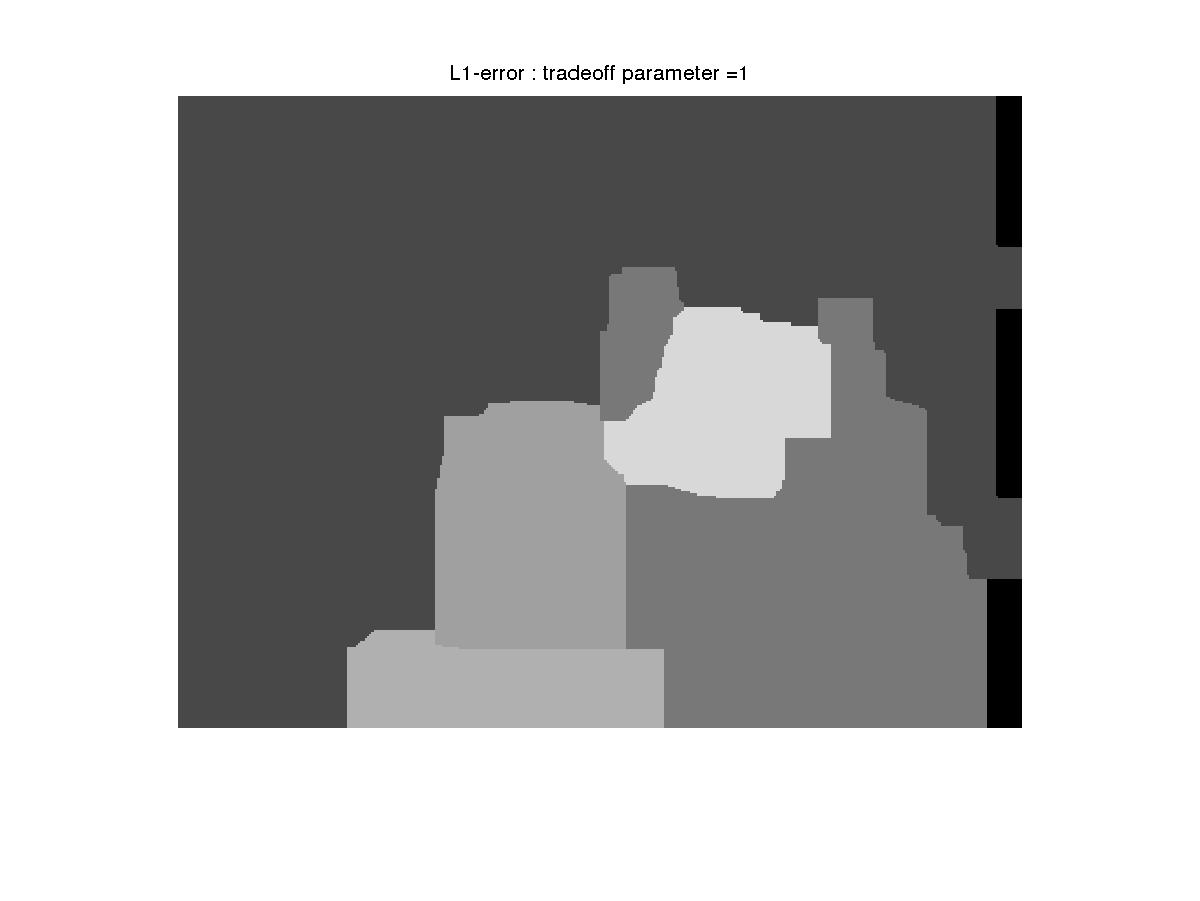
\includegraphics[scale=0.2]{./pics/tsukuba_L1_error_p=1.jpg}
\caption{L1 error with p=1}
\end{subfigure}
 \begin{subfigure}{0.5\textwidth}
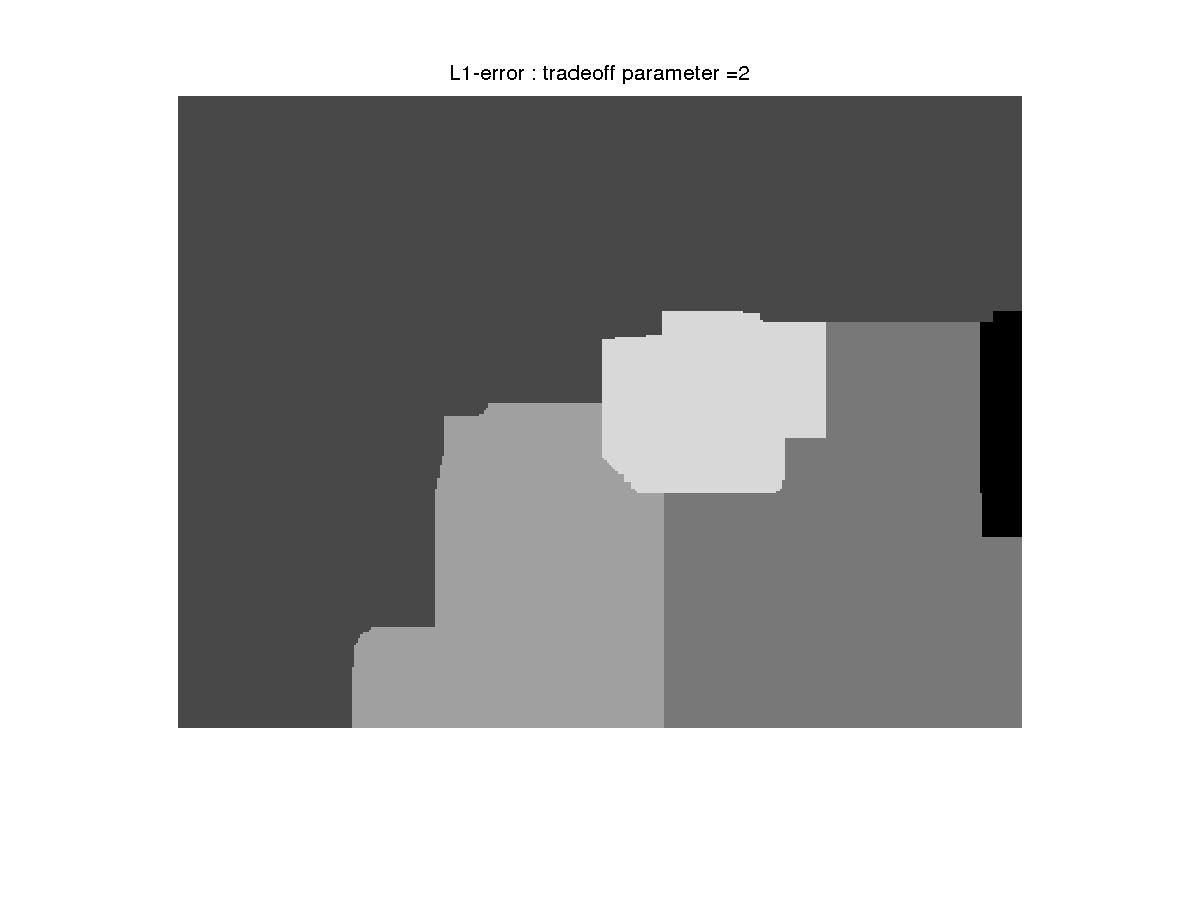
\includegraphics[scale=0.2]{./pics/tsukuba_L1_error_p=2.jpg}
\caption{L1 error with p=2}
\end{subfigure}
 \begin{subfigure}{0.5\textwidth}
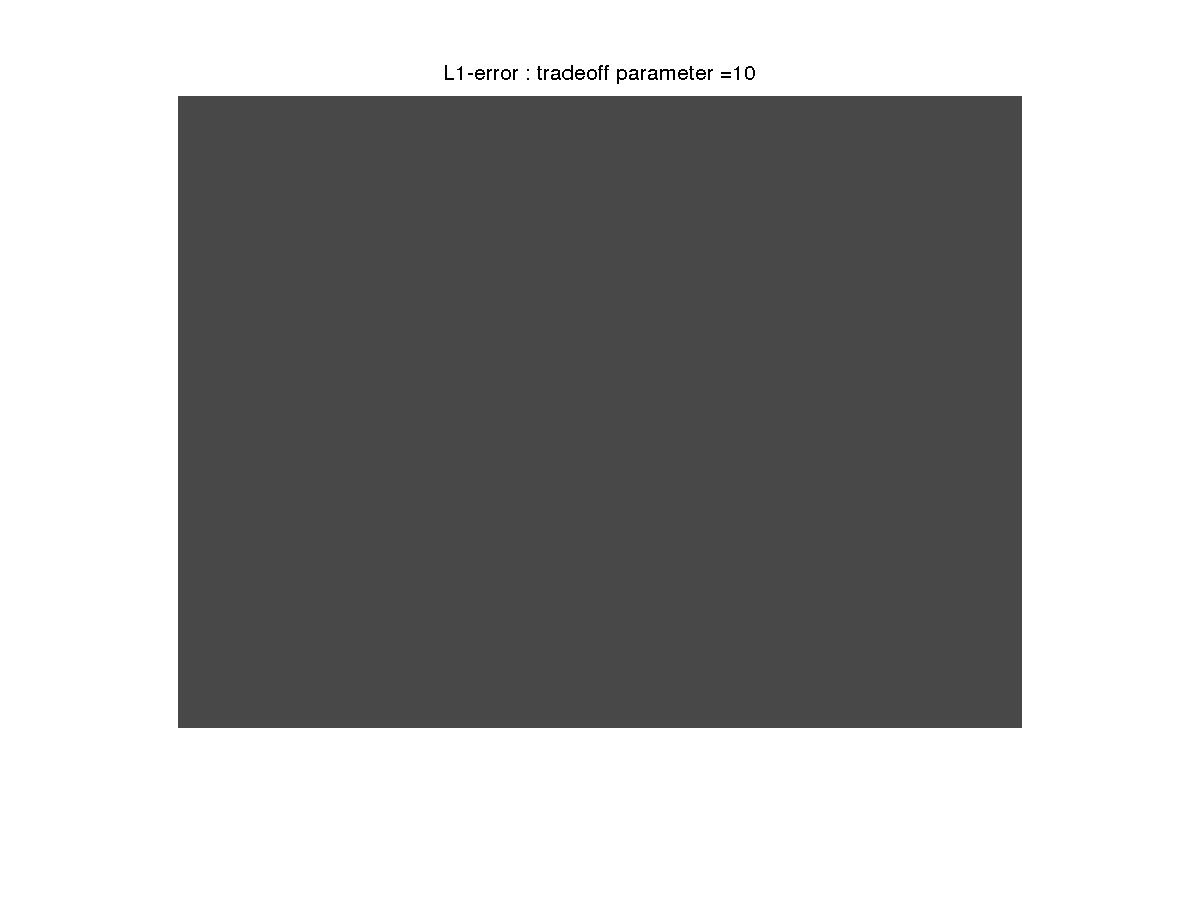
\includegraphics[scale=0.2]{./pics/tsukuba_L1_error_p=10.jpg}
\caption{L1 error with p=10}
\end{subfigure}
\end{figure}
from the figures, the best value for p is found to be 0.1.

\clearpage
\subsubsection{L2 cost function}
\begin{figure}[!ht]
 \begin{subfigure}{0.5\textwidth}
 \centering
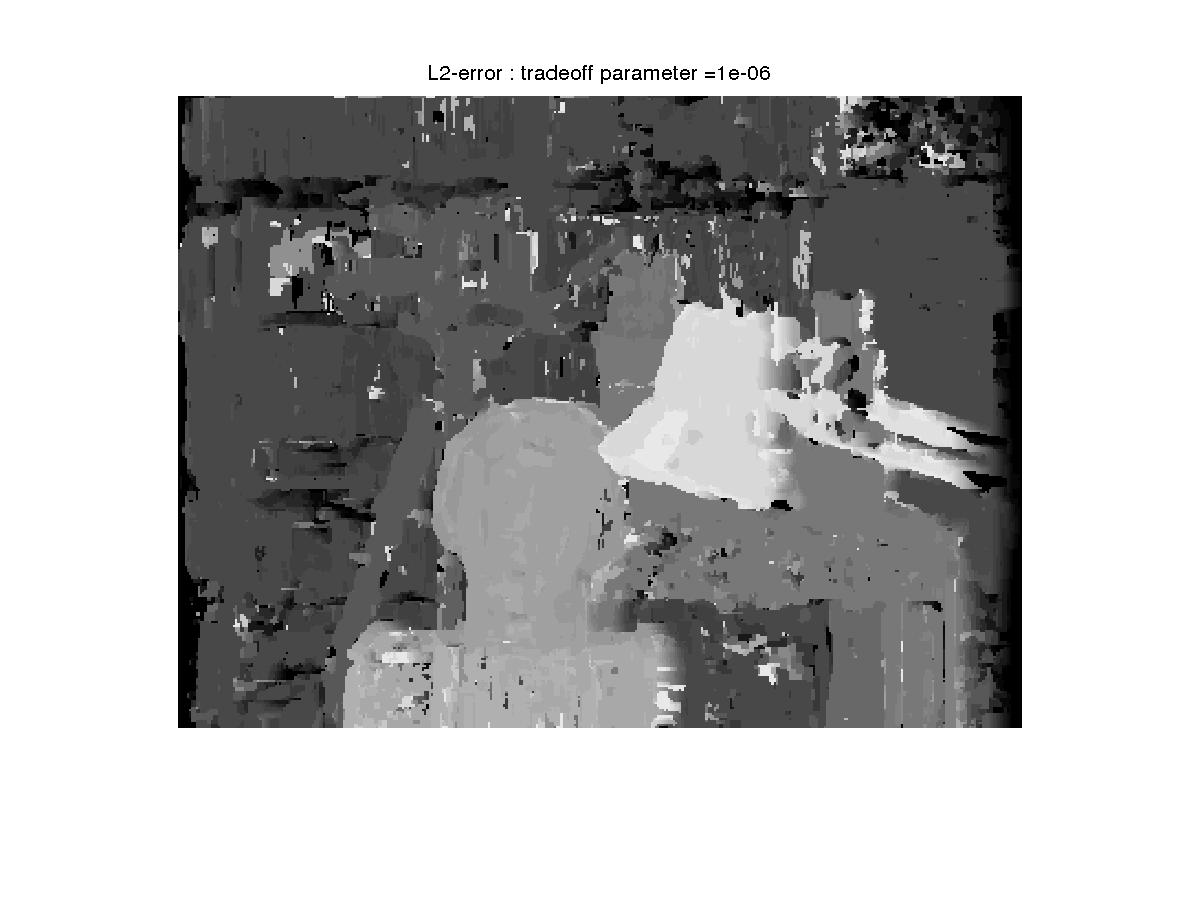
\includegraphics[scale=0.2]{./pics/tsukuba_L2_error_p=1e-06.jpg}
\caption{L2 error with p=1e-6}
\end{subfigure}
 \begin{subfigure}{0.5\textwidth}
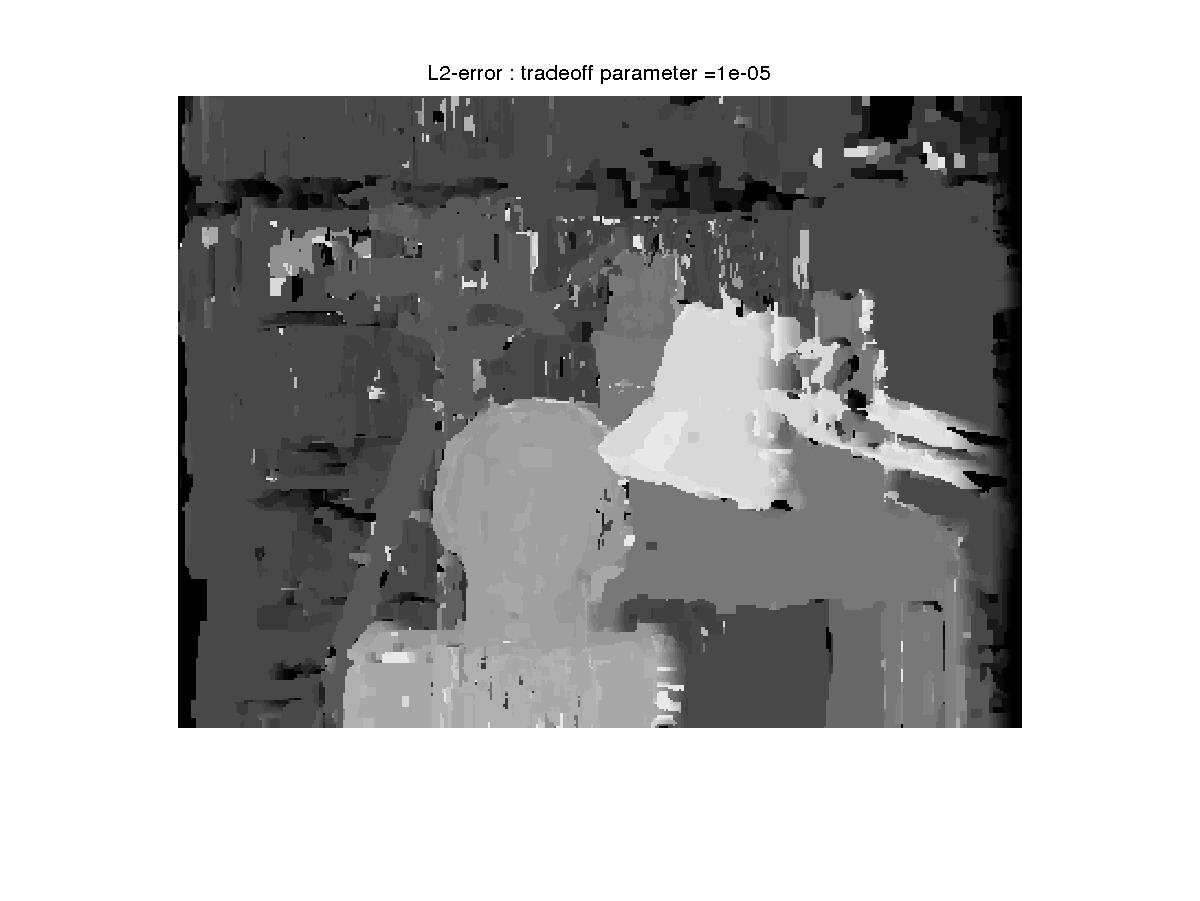
\includegraphics[scale=0.2]{./pics/tsukuba_L2_error_p=1e-05.jpg}
\caption{L2 error with p=1e-5}
\end{subfigure}
 \begin{subfigure}{0.5\textwidth}
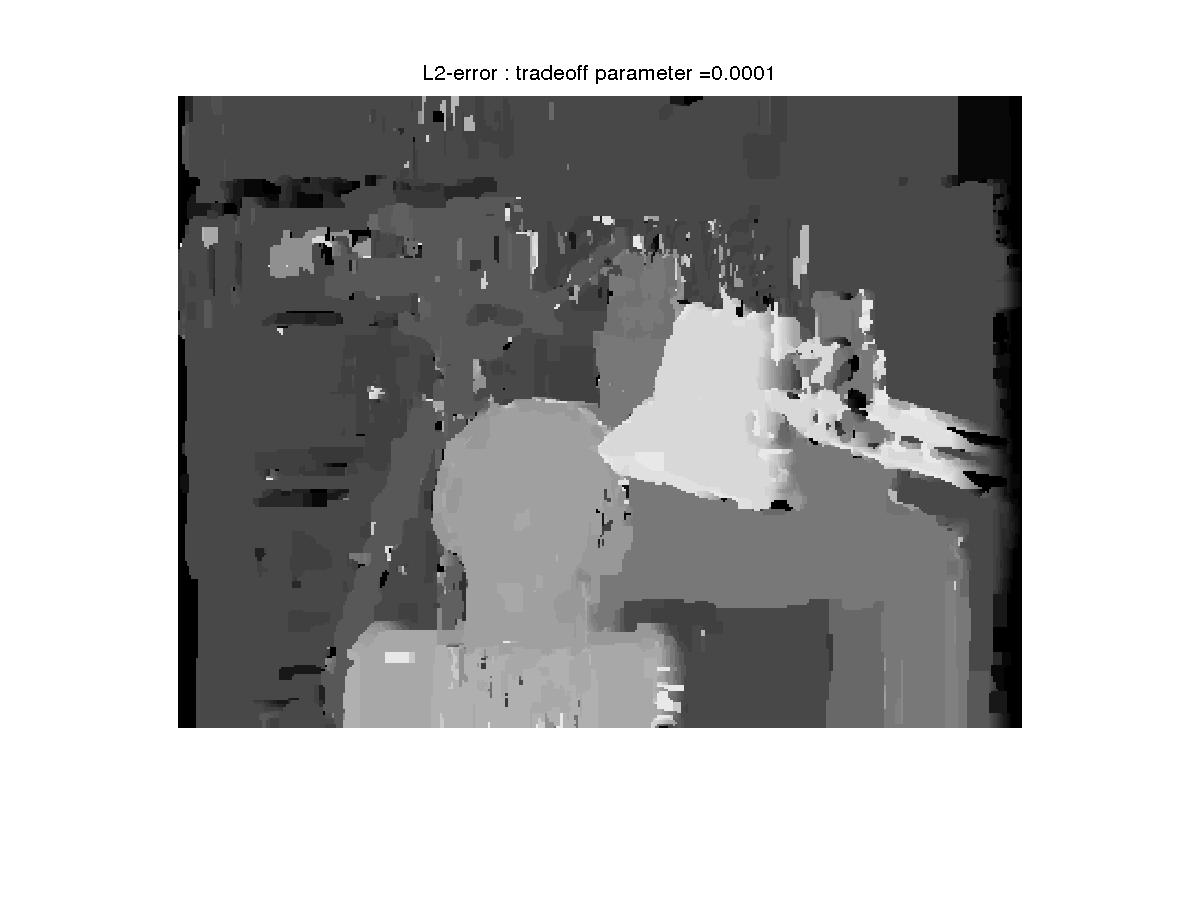
\includegraphics[scale=0.2]{./pics/tsukuba_L2_error_p=0.0001.jpg}
\caption{L2 error with p=0.0001}
\end{subfigure}
 \begin{subfigure}{0.5\textwidth}
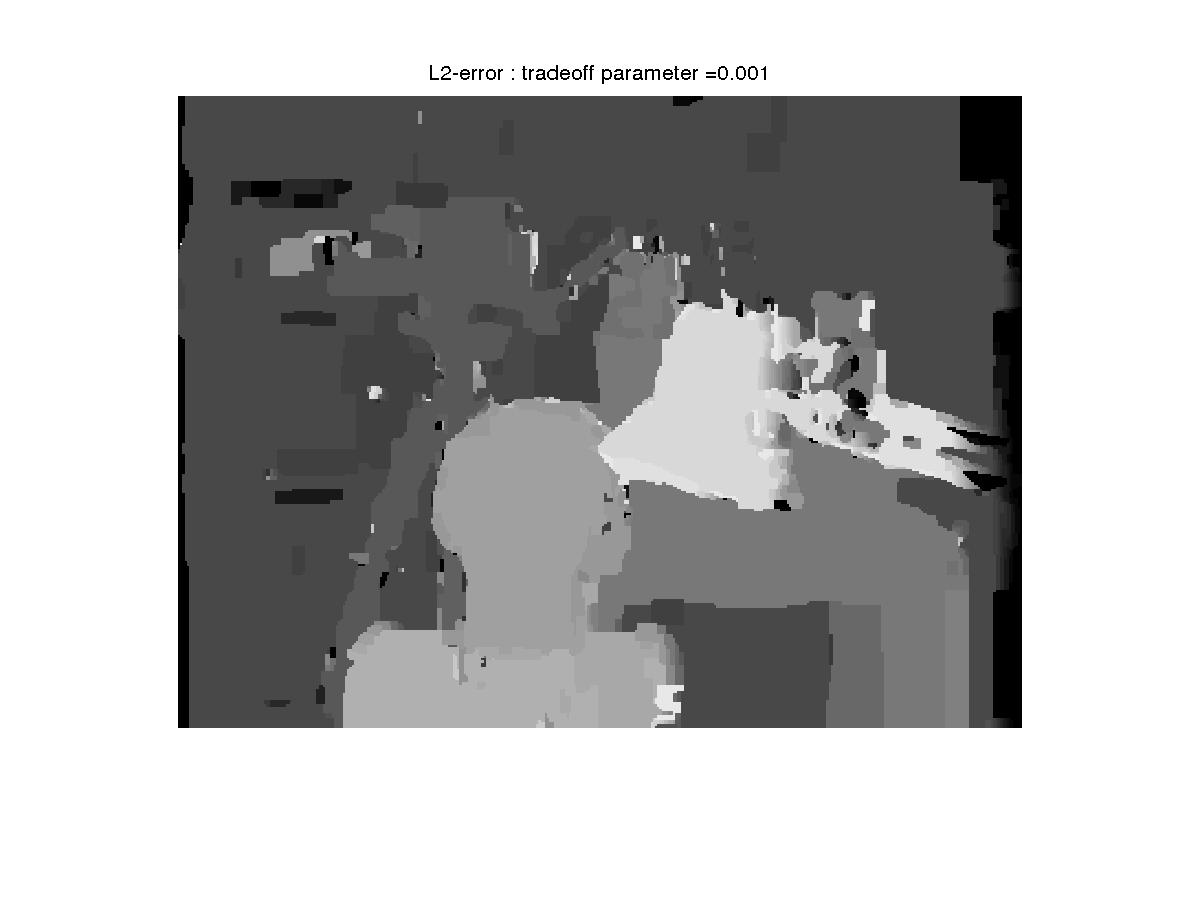
\includegraphics[scale=0.2]{./pics/tsukuba_L2_error_p=0.001.jpg}
\caption{L2 error with p=0.001}
\end{subfigure}
 \begin{subfigure}{0.5\textwidth}
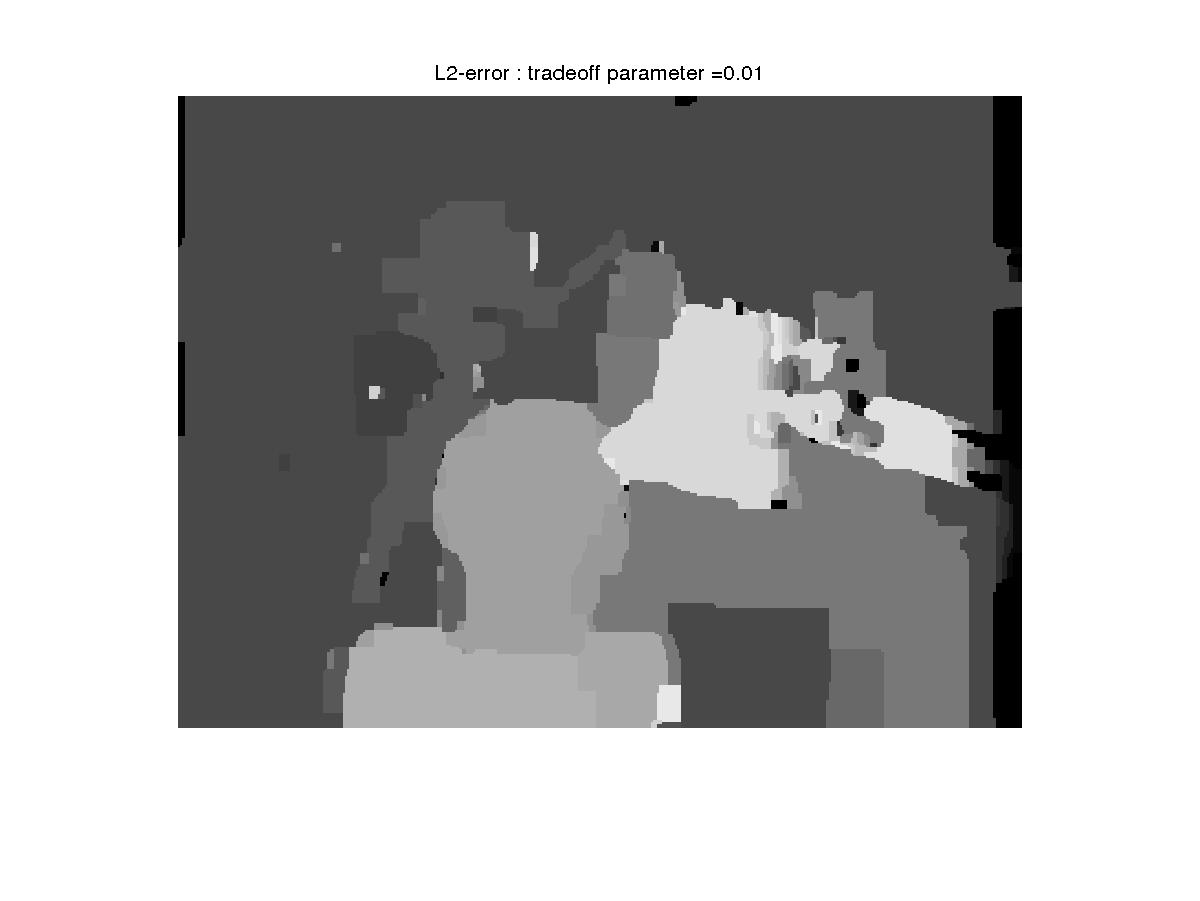
\includegraphics[scale=0.2]{./pics/tsukuba_L2_error_p=0.01.jpg}
\caption{L2 error with p=0.01}
\end{subfigure}
 \begin{subfigure}{0.5\textwidth}
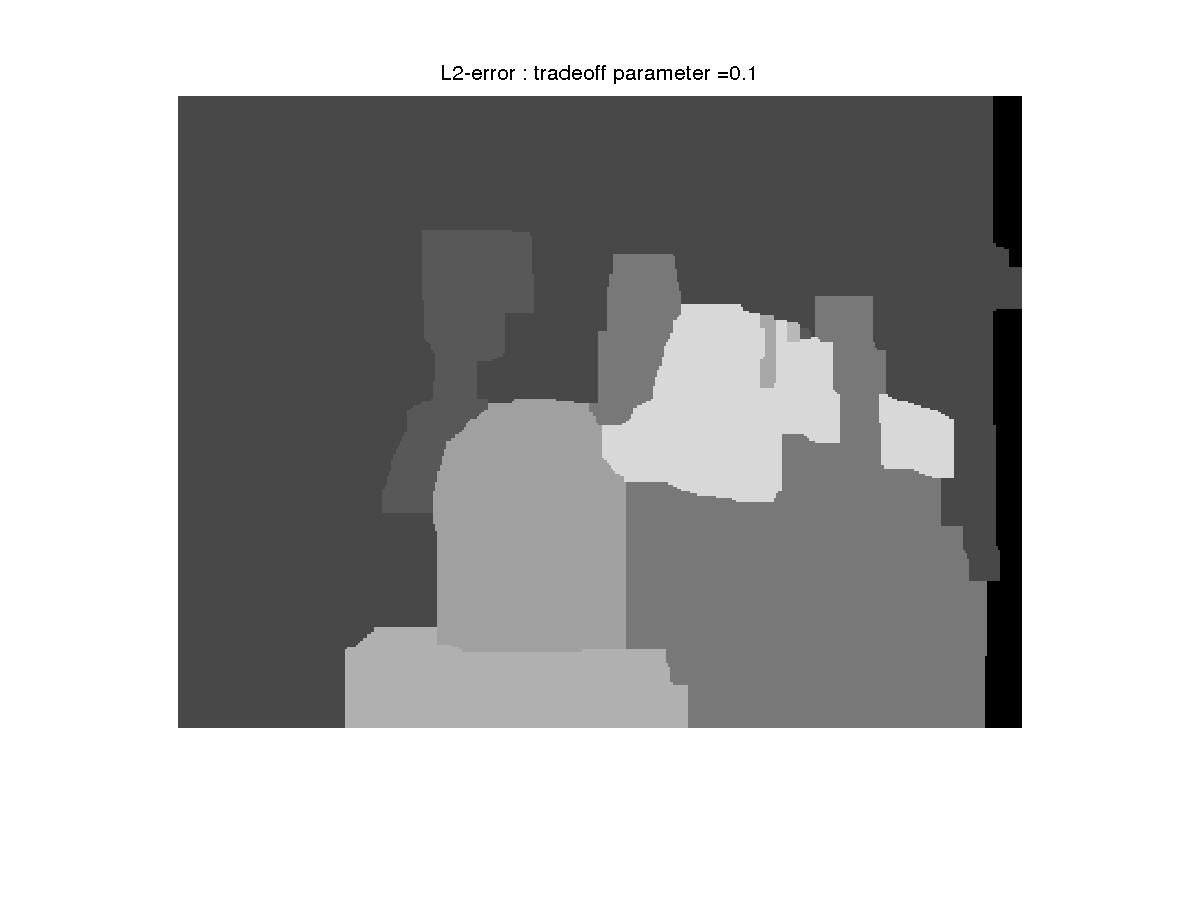
\includegraphics[scale=0.2]{./pics/tsukuba_L2_error_p=0.1.jpg}
\caption{L2 error with p=0.1}
\end{subfigure}
\end{figure}
\begin{figure}
 \begin{subfigure}{0.5\textwidth}
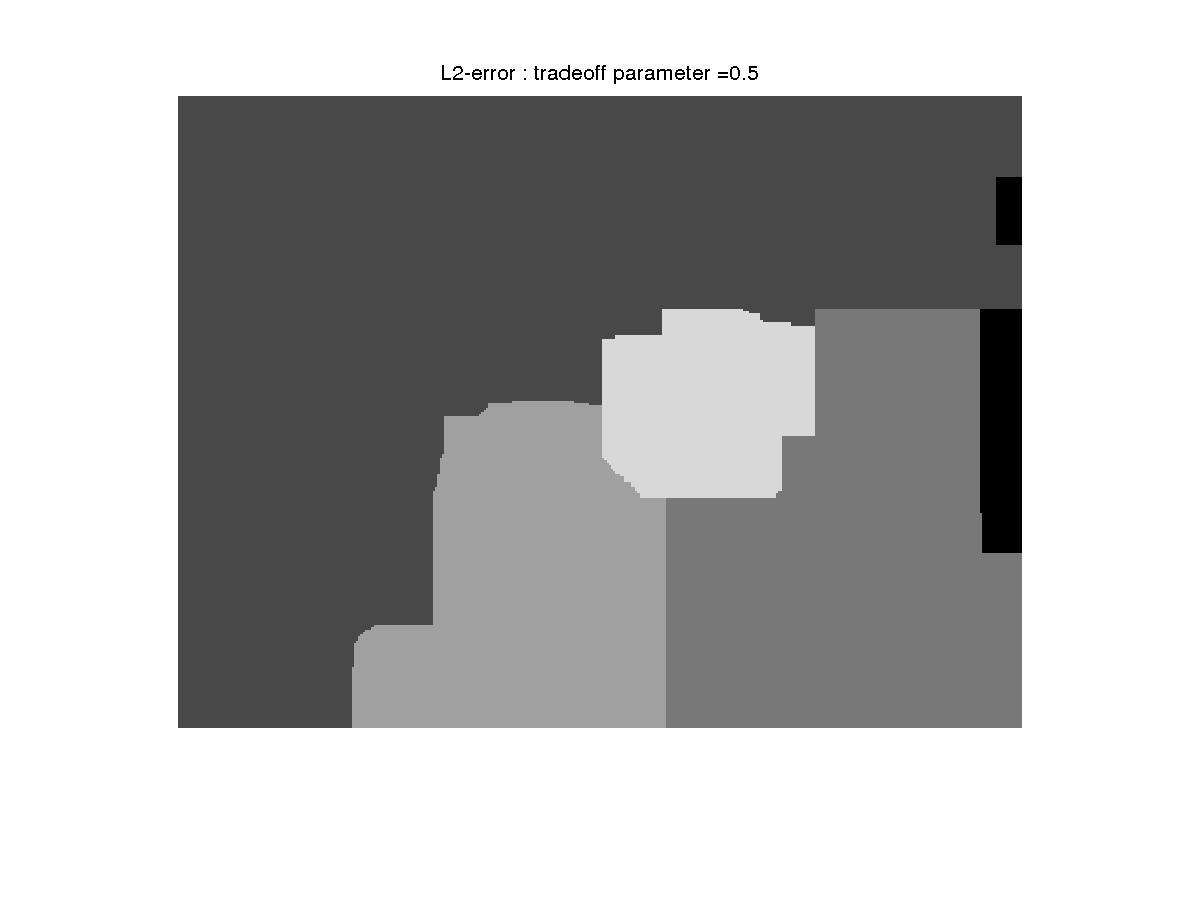
\includegraphics[scale=0.2]{./pics/tsukuba_L2_error_p=0.5.jpg}
\caption{L2 error with p=0.5}
\end{subfigure}
 \begin{subfigure}{0.5\textwidth}
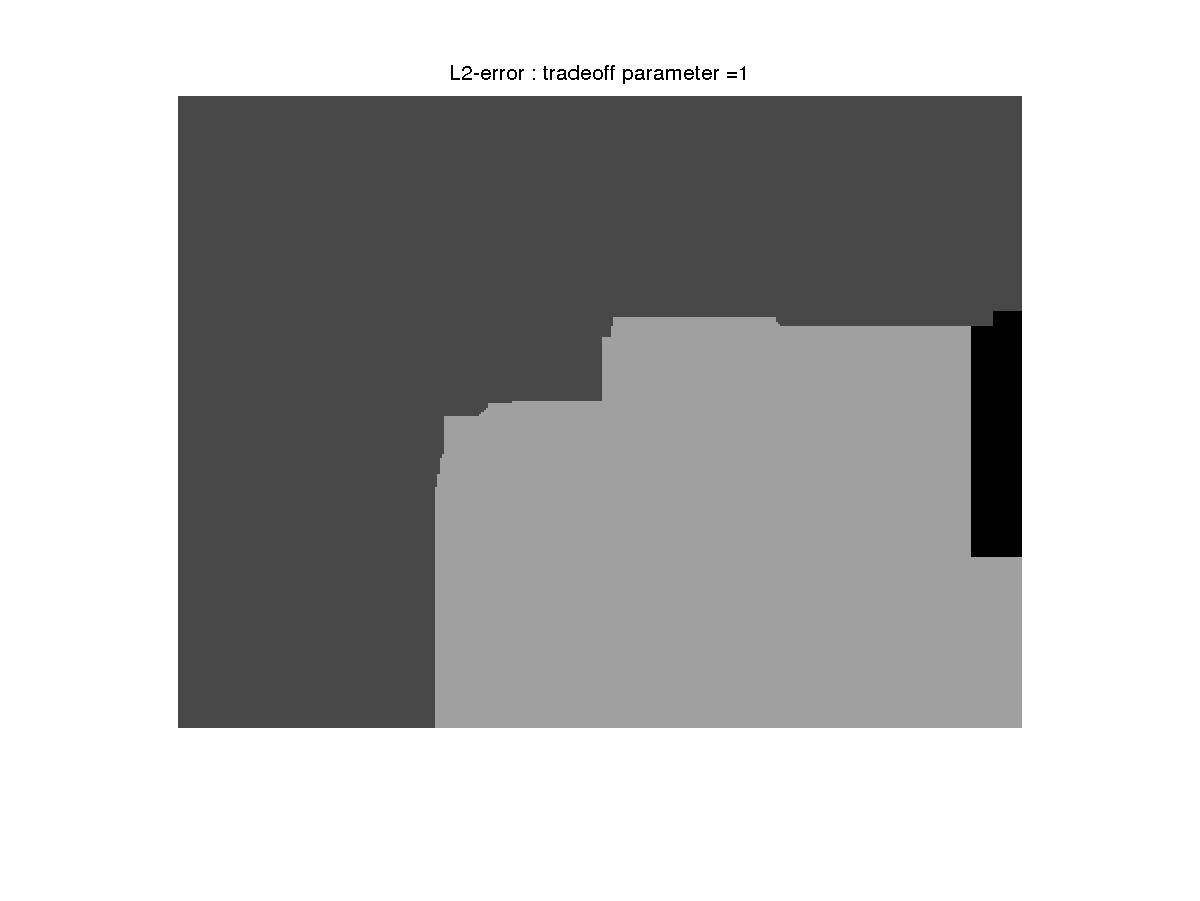
\includegraphics[scale=0.2]{./pics/tsukuba_L2_error_p=1.jpg}
\caption{L2 error with p=1}
\end{subfigure}
 \begin{subfigure}{0.5\textwidth}
\includegraphics[scale=0.2]{./pics/tsukuba_L2_error_p=2.jpg}
\caption{L2 error with p=2}
\end{subfigure}
 \begin{subfigure}{0.5\textwidth}
\includegraphics[scale=0.2]{./pics/tsukuba_L2_error_p=10.jpg}
\caption{L2 error with p=10}
\end{subfigure}
\end{figure}
from the figures, the best value for p is found to be 0.01.

\end{document}